% This file was converted to LaTeX by Writer2LaTeX ver. 1.4
% see http://writer2latex.sourceforge.net for more info
\documentclass[12pt]{article}
\usepackage[utf8]{inputenc}
\usepackage[T1]{fontenc}
\usepackage[english]{babel}
\usepackage{amsmath}
\usepackage{amssymb,amsfonts,textcomp}
\usepackage{array}
\usepackage{hhline}
\usepackage{hyperref}
\hypersetup{colorlinks=true, linkcolor=blue, citecolor=blue, filecolor=blue, urlcolor=blue}
\usepackage{graphicx}
% footnotes configuration
\makeatletter
\renewcommand\thefootnote{\arabic{footnote}}
\renewcommand\@makefnmark{\mbox{\textstyleFootnoteanchor{\@thefnmark}}}
\makeatother
\newcommand\textsubscript[1]{\ensuremath{{}_{\text{#1}}}}
% Text styles
\newcommand\textstyleFootnoteSymbol[1]{{\fontsize{6.5pt}{7.8pt}\selectfont #1}}
\newcommand\textstyleInternetlink[1]{#1}
\newcommand\textstyleFootnoteanchor[1]{{\fontsize{6.5pt}{7.8pt}\selectfont \textsuperscript{#1}}}
\raggedbottom
% Paragraph styles
\renewcommand\familydefault{\rmdefault}
\newenvironment{styleStandard}{\setlength\leftskip{0cm}\setlength\rightskip{0cm plus 1fil}\setlength\parindent{0cm}\setlength\parfillskip{0pt plus 1fil}\setlength\parskip{0in plus 1pt}\writerlistparindent\writerlistleftskip\leavevmode\normalfont\normalsize\writerlistlabel\ignorespaces}{\unskip\vspace{0.111in plus 0.0111in}\par}
\newenvironment{stylelsSectioni}{\setlength\leftskip{0.25in}\setlength\rightskip{0in plus 1fil}\setlength\parindent{0in}\setlength\parfillskip{0pt plus 1fil}\setlength\parskip{0.1665in plus 0.016649999in}\writerlistparindent\writerlistleftskip\leavevmode\normalfont\normalsize\fontsize{18pt}{21.6pt}\selectfont\bfseries\writerlistlabel\ignorespaces}{\unskip\vspace{0.0835in plus 0.00835in}\par}
\newenvironment{stylelsSectionii}{\setlength\leftskip{0.248in}\setlength\rightskip{0in plus 1fil}\setlength\parindent{-0.248in}\setlength\parfillskip{0pt plus 1fil}\setlength\parskip{0.222in plus 0.0222in}\writerlistparindent\writerlistleftskip\leavevmode\normalfont\normalsize\fontsize{16pt}{19.2pt}\selectfont\bfseries\writerlistlabel\ignorespaces}{\unskip\vspace{0.0835in plus 0.00835in}\par}
\newenvironment{styleListParagraph}{\renewcommand\baselinestretch{1.0}\setlength\leftskip{0.5in}\setlength\rightskip{0in plus 1fil}\setlength\parindent{0in}\setlength\parfillskip{0pt plus 1fil}\setlength\parskip{0in plus 1pt}\writerlistparindent\writerlistleftskip\leavevmode\normalfont\normalsize\fontsize{11pt}{13.2pt}\selectfont\writerlistlabel\ignorespaces}{\unskip\vspace{0.111in plus 0.0111in}\par}
\newenvironment{styleFootnote}{\setlength\leftskip{0.2354in}\setlength\rightskip{0in plus 1fil}\setlength\parindent{-0.2354in}\setlength\parfillskip{0pt plus 1fil}\setlength\parskip{0in plus 1pt}\writerlistparindent\writerlistleftskip\leavevmode\normalfont\normalsize\fontsize{10pt}{12.0pt}\selectfont\writerlistlabel\ignorespaces}{\unskip\vspace{0.111in plus 0.0111in}\par}
\newenvironment{styleTextbody}{\renewcommand\baselinestretch{1.0}\setlength\leftskip{0cm}\setlength\rightskip{0cm plus 1fil}\setlength\parindent{0cm}\setlength\parfillskip{0pt plus 1fil}\setlength\parskip{0in plus 1pt}\writerlistparindent\writerlistleftskip\leavevmode\normalfont\normalsize\fontsize{11pt}{13.2pt}\selectfont\writerlistlabel\ignorespaces}{\unskip\vspace{0.0835in plus 0.00835in}\par}
\newenvironment{styleNormalWeb}{\setlength\leftskip{0cm}\setlength\rightskip{0cm plus 1fil}\setlength\parindent{0cm}\setlength\parfillskip{0pt plus 1fil}\setlength\parskip{0in plus 1pt}\writerlistparindent\writerlistleftskip\leavevmode\normalfont\normalsize\writerlistlabel\ignorespaces}{\unskip\vspace{0.111in plus 0.0111in}\par}
% List styles
\newcommand\writerlistleftskip{}
\newcommand\writerlistparindent{}
\newcommand\writerlistlabel{}
\newcommand\writerlistremovelabel{\aftergroup\let\aftergroup\writerlistparindent\aftergroup\relax\aftergroup\let\aftergroup\writerlistlabel\aftergroup\relax}
\newcounter{listWWNumxxiileveli}
\newcounter{listWWNumxxiilevelii}[listWWNumxxiileveli]
\newcounter{listWWNumxxiileveliii}[listWWNumxxiilevelii]
\newcounter{listWWNumxxiileveliv}[listWWNumxxiileveliii]
\renewcommand\thelistWWNumxxiileveli{\arabic{listWWNumxxiileveli}}
\renewcommand\thelistWWNumxxiilevelii{\arabic{listWWNumxxiileveli}.\arabic{listWWNumxxiilevelii}}
\renewcommand\thelistWWNumxxiileveliii{\arabic{listWWNumxxiileveli}.\arabic{listWWNumxxiilevelii}.\arabic{listWWNumxxiileveliii}}
\renewcommand\thelistWWNumxxiileveliv{\arabic{listWWNumxxiileveli}.\arabic{listWWNumxxiilevelii}.\arabic{listWWNumxxiileveliii}.\arabic{listWWNumxxiileveliv}}
\newcommand\labellistWWNumxxiileveli{\thelistWWNumxxiileveli.}
\newcommand\labellistWWNumxxiilevelii{\thelistWWNumxxiilevelii.}
\newcommand\labellistWWNumxxiileveliii{\thelistWWNumxxiileveliii.}
\newcommand\labellistWWNumxxiileveliv{\thelistWWNumxxiileveliv.}
\newenvironment{listWWNumxxiileveli}{\def\writerlistleftskip{\setlength\leftskip{0.5in}}\def\writerlistparindent{}\def\writerlistlabel{}\def\item{\def\writerlistparindent{\setlength\parindent{-0.25in}}\def\writerlistlabel{\stepcounter{listWWNumxxiileveli}\makebox[0cm][l]{\labellistWWNumxxiileveli}\hspace{-0.635cm}\writerlistremovelabel}}}{}
\newenvironment{listWWNumxxiilevelii}{\def\writerlistleftskip{\setlength\leftskip{1in}}\def\writerlistparindent{}\def\writerlistlabel{}\def\item{\def\writerlistparindent{\setlength\parindent{-0.25in}}\def\writerlistlabel{\stepcounter{listWWNumxxiilevelii}\makebox[0cm][l]{\labellistWWNumxxiilevelii}\hspace{-1.905cm}\writerlistremovelabel}}}{}
\newenvironment{listWWNumxxiileveliii}{\def\writerlistleftskip{\setlength\leftskip{1.5in}}\def\writerlistparindent{}\def\writerlistlabel{}\def\item{\def\writerlistparindent{\setlength\parindent{-0.1252in}}\def\writerlistlabel{\stepcounter{listWWNumxxiileveliii}\makebox[0cm][r]{\labellistWWNumxxiileveliii}\hspace{-3.4919918cm}\writerlistremovelabel}}}{}
\newenvironment{listWWNumxxiileveliv}{\def\writerlistleftskip{\setlength\leftskip{2in}}\def\writerlistparindent{}\def\writerlistlabel{}\def\item{\def\writerlistparindent{\setlength\parindent{-0.25in}}\def\writerlistlabel{\stepcounter{listWWNumxxiileveliv}\makebox[0cm][l]{\labellistWWNumxxiileveliv}\hspace{-4.4449997cm}\writerlistremovelabel}}}{}
\newcounter{listWWNumxxviiileveli}
\newcounter{listWWNumxxviiilevelii}[listWWNumxxviiileveli]
\newcounter{listWWNumxxviiileveliii}[listWWNumxxviiilevelii]
\newcounter{listWWNumxxviiileveliv}[listWWNumxxviiileveliii]
\renewcommand\thelistWWNumxxviiileveli{\arabic{listWWNumxxviiileveli}}
\renewcommand\thelistWWNumxxviiilevelii{\alph{listWWNumxxviiilevelii}}
\renewcommand\thelistWWNumxxviiileveliii{\roman{listWWNumxxviiileveliii}}
\renewcommand\thelistWWNumxxviiileveliv{\arabic{listWWNumxxviiileveliv}}
\newcommand\labellistWWNumxxviiileveli{\thelistWWNumxxviiileveli.}
\newcommand\labellistWWNumxxviiilevelii{\thelistWWNumxxviiilevelii.}
\newcommand\labellistWWNumxxviiileveliii{\thelistWWNumxxviiileveliii.}
\newcommand\labellistWWNumxxviiileveliv{\thelistWWNumxxviiileveliv.}
\newenvironment{listWWNumxxviiileveli}{\def\writerlistleftskip{\setlength\leftskip{0.5in}}\def\writerlistparindent{}\def\writerlistlabel{}\def\item{\def\writerlistparindent{\setlength\parindent{-0.25in}}\def\writerlistlabel{\stepcounter{listWWNumxxviiileveli}\makebox[0cm][l]{\labellistWWNumxxviiileveli}\hspace{-0.635cm}\writerlistremovelabel}}}{}
\newenvironment{listWWNumxxviiilevelii}{\def\writerlistleftskip{\setlength\leftskip{1in}}\def\writerlistparindent{}\def\writerlistlabel{}\def\item{\def\writerlistparindent{\setlength\parindent{-0.25in}}\def\writerlistlabel{\stepcounter{listWWNumxxviiilevelii}\makebox[0cm][l]{\labellistWWNumxxviiilevelii}\hspace{-1.905cm}\writerlistremovelabel}}}{}
\newenvironment{listWWNumxxviiileveliii}{\def\writerlistleftskip{\setlength\leftskip{1.5in}}\def\writerlistparindent{}\def\writerlistlabel{}\def\item{\def\writerlistparindent{\setlength\parindent{-0.1252in}}\def\writerlistlabel{\stepcounter{listWWNumxxviiileveliii}\makebox[0cm][r]{\labellistWWNumxxviiileveliii}\hspace{-3.4919918cm}\writerlistremovelabel}}}{}
\newenvironment{listWWNumxxviiileveliv}{\def\writerlistleftskip{\setlength\leftskip{2in}}\def\writerlistparindent{}\def\writerlistlabel{}\def\item{\def\writerlistparindent{\setlength\parindent{-0.25in}}\def\writerlistlabel{\stepcounter{listWWNumxxviiileveliv}\makebox[0cm][l]{\labellistWWNumxxviiileveliv}\hspace{-4.4449997cm}\writerlistremovelabel}}}{}
\newcounter{listWWNumxxvleveli}
\newcounter{listWWNumxxvlevelii}[listWWNumxxvleveli]
\newcounter{listWWNumxxvleveliii}[listWWNumxxvlevelii]
\newcounter{listWWNumxxvleveliv}[listWWNumxxvleveliii]
\renewcommand\thelistWWNumxxvleveli{\roman{listWWNumxxvleveli}}
\renewcommand\thelistWWNumxxvlevelii{\alph{listWWNumxxvlevelii}}
\renewcommand\thelistWWNumxxvleveliii{\roman{listWWNumxxvleveliii}}
\renewcommand\thelistWWNumxxvleveliv{\arabic{listWWNumxxvleveliv}}
\newcommand\labellistWWNumxxvleveli{(\thelistWWNumxxvleveli)}
\newcommand\labellistWWNumxxvlevelii{\thelistWWNumxxvlevelii.}
\newcommand\labellistWWNumxxvleveliii{\thelistWWNumxxvleveliii.}
\newcommand\labellistWWNumxxvleveliv{\thelistWWNumxxvleveliv.}
\newenvironment{listWWNumxxvleveli}{\def\writerlistleftskip{\setlength\leftskip{0.5in}}\def\writerlistparindent{}\def\writerlistlabel{}\def\item{\def\writerlistparindent{\setlength\parindent{-0.5in}}\def\writerlistlabel{\stepcounter{listWWNumxxvleveli}\makebox[0cm][l]{\labellistWWNumxxvleveli}\hspace{0.0cm}\writerlistremovelabel}}}{}
\newenvironment{listWWNumxxvlevelii}{\def\writerlistleftskip{\setlength\leftskip{0.75in}}\def\writerlistparindent{}\def\writerlistlabel{}\def\item{\def\writerlistparindent{\setlength\parindent{-0.25in}}\def\writerlistlabel{\stepcounter{listWWNumxxvlevelii}\makebox[0cm][l]{\labellistWWNumxxvlevelii}\hspace{-1.27cm}\writerlistremovelabel}}}{}
\newenvironment{listWWNumxxvleveliii}{\def\writerlistleftskip{\setlength\leftskip{1.25in}}\def\writerlistparindent{}\def\writerlistlabel{}\def\item{\def\writerlistparindent{\setlength\parindent{-0.1252in}}\def\writerlistlabel{\stepcounter{listWWNumxxvleveliii}\makebox[0cm][r]{\labellistWWNumxxvleveliii}\hspace{-2.8569918cm}\writerlistremovelabel}}}{}
\newenvironment{listWWNumxxvleveliv}{\def\writerlistleftskip{\setlength\leftskip{1.75in}}\def\writerlistparindent{}\def\writerlistlabel{}\def\item{\def\writerlistparindent{\setlength\parindent{-0.25in}}\def\writerlistlabel{\stepcounter{listWWNumxxvleveliv}\makebox[0cm][l]{\labellistWWNumxxvleveliv}\hspace{-3.81cm}\writerlistremovelabel}}}{}
\newcounter{listWWNumxxvileveli}
\newcounter{listWWNumxxvilevelii}[listWWNumxxvileveli]
\newcounter{listWWNumxxvileveliii}[listWWNumxxvilevelii]
\newcounter{listWWNumxxvileveliv}[listWWNumxxvileveliii]
\renewcommand\thelistWWNumxxvileveli{\roman{listWWNumxxvileveli}}
\renewcommand\thelistWWNumxxvilevelii{\alph{listWWNumxxvilevelii}}
\renewcommand\thelistWWNumxxvileveliii{\roman{listWWNumxxvileveliii}}
\renewcommand\thelistWWNumxxvileveliv{\arabic{listWWNumxxvileveliv}}
\newcommand\labellistWWNumxxvileveli{(\thelistWWNumxxvileveli)}
\newcommand\labellistWWNumxxvilevelii{\thelistWWNumxxvilevelii.}
\newcommand\labellistWWNumxxvileveliii{\thelistWWNumxxvileveliii.}
\newcommand\labellistWWNumxxvileveliv{\thelistWWNumxxvileveliv.}
\newenvironment{listWWNumxxvileveli}{\def\writerlistleftskip{\setlength\leftskip{0.75in}}\def\writerlistparindent{}\def\writerlistlabel{}\def\item{\def\writerlistparindent{\setlength\parindent{-0.5in}}\def\writerlistlabel{\stepcounter{listWWNumxxvileveli}\makebox[0cm][l]{\labellistWWNumxxvileveli}\hspace{-0.635cm}\writerlistremovelabel}}}{}
\newenvironment{listWWNumxxvilevelii}{\def\writerlistleftskip{\setlength\leftskip{1in}}\def\writerlistparindent{}\def\writerlistlabel{}\def\item{\def\writerlistparindent{\setlength\parindent{-0.25in}}\def\writerlistlabel{\stepcounter{listWWNumxxvilevelii}\makebox[0cm][l]{\labellistWWNumxxvilevelii}\hspace{-1.905cm}\writerlistremovelabel}}}{}
\newenvironment{listWWNumxxvileveliii}{\def\writerlistleftskip{\setlength\leftskip{1.5in}}\def\writerlistparindent{}\def\writerlistlabel{}\def\item{\def\writerlistparindent{\setlength\parindent{-0.1252in}}\def\writerlistlabel{\stepcounter{listWWNumxxvileveliii}\makebox[0cm][r]{\labellistWWNumxxvileveliii}\hspace{-3.4919918cm}\writerlistremovelabel}}}{}
\newenvironment{listWWNumxxvileveliv}{\def\writerlistleftskip{\setlength\leftskip{2in}}\def\writerlistparindent{}\def\writerlistlabel{}\def\item{\def\writerlistparindent{\setlength\parindent{-0.25in}}\def\writerlistlabel{\stepcounter{listWWNumxxvileveliv}\makebox[0cm][l]{\labellistWWNumxxvileveliv}\hspace{-4.4449997cm}\writerlistremovelabel}}}{}
\title{}
\author{Anna}
\date{2019-06-18}
\begin{document}
\title{\textsuperscript{Datives as applicatives}\footnote{\textstyleFootnoteSymbol{*} I thank two anonymous reviewers for useful comments and suggestions. I am also grateful to Taylor Roberts and the editors of this volume. This work was supported by a Jackman Humanities Institute Fellowship. }}
\maketitle

\begin{styleStandard}
\textbf{María Cristina Cuervo}
\end{styleStandard}

\begin{styleStandard}
\textbf{University of Toronto}
\end{styleStandard}

\begin{styleStandard}
\textbf{\textit{Abstract}}\textit{: This work investigates dative arguments within a theory of applicative arguments. The focus is on what dative arguments have in common as a class—well beyond the most typical datives in ditransitive constructions—and as subcases of applied arguments, as found in both languages with a rich case system, and languages without overt case marking.}
\end{styleStandard}

\begin{styleStandard}
\textit{A typology of applicative constructions that directly associates with dative arguments is developed. The various subtypes of applicatives are derived from a restricted set of structural properties and syntactic-semantic features (the type of complement of the Appl head, the dynamic/stative nature of its complement, and the presence/absence of an external argument, and of a verbal head above the applicative).}
\end{styleStandard}

\begin{styleStandard}
\textit{The various interpretations of applied arguments (e.g., possessors, bene/malefactives, recipients, experiencers, affected, causees) are configurationally derived, and do not require encoding as part of the denotation of the applicative head beyond the traditional, minimal notion of Appl as introducing an argument “oriented” towards its complement. This richness of interpretations sets applied arguments apart from the narrow range of interpretations for arguments of v/Voice, on the one hand, and the practically unconstrained interpretations of arguments of lexical verbs/roots, on the other. }
\end{styleStandard}

\begin{styleStandard}
\textbf{\textit{Keywords: }}\textit{\ dative arguments, applicatives, experiencers, possessors}
\end{styleStandard}


\setcounter{listWWNumxxiileveli}{0}
\begin{listWWNumxxiileveli}
\item 
\begin{stylelsSectioni}
Datives and applicatives
\end{stylelsSectioni}


\setcounter{listWWNumxxiilevelii}{0}
\begin{listWWNumxxiilevelii}
\item 
\begin{stylelsSectionii}
Introduction
\end{stylelsSectionii}
\end{listWWNumxxiilevelii}
\end{listWWNumxxiileveli}
\begin{styleStandard}
Dative arguments appear in many languages as the third morphological case, after nominative and accusative, or ergative and absolutive. Although the most common role of datives seems to be that of indirect object with transitive verbs—typically as recipients—arguments in dative case can combine with all classes of predicates, and can express sources, experiencers, possessors, benefactives, malefactives, causees, locations, affectees, non-volitional agents or dispositionals. Both inter- and intra-linguistically a dative argument can alternate with accusative, genitive, and nominative DPs, or with prepositional phrases. 
\end{styleStandard}

\begin{styleStandard}
It is possible to consider that such variety of meanings and constructions prevents us from finding a common core, and that dative case can be unpredictable, or a default case. \ There has been, however, a lot of work seeking unification either at the semantic or the syntactic levels. Sometimes the unification has proposed that all true datives are extensions of prototypical indirect objects in ditransitive constructions. 
\end{styleStandard}

\begin{styleStandard}
In this work I present an approach to the investigation of dative arguments within a theory of applicative arguments. In order to develop this approach, I start with the hypothesis that dative arguments are applicative arguments, and focus on the syntactic context into which an applicative head is merged, with particular attention to certain properties of the complement and the head that selects the applicative phrase. This is done for two reasons:
\end{styleStandard}


\setcounter{listWWNumxxviiileveli}{0}
\begin{listWWNumxxviiileveli}
\item 
\begin{styleListParagraph}
the belief that both the complement structure and the structure immediately above the applicative are relevant for a typology of applicative constructions that accounts for their syntax and provides a base on which to develop a systematic account of their crosslinguistic distribution.
\end{styleListParagraph}
\item 
\begin{styleListParagraph}
the belief that dative/applicative arguments—like subjects and unlike direct objects—have structural meanings; that is, that their interpretation is predictable (beyond certain idiosyncrasies related to the meaning of verbal roots) on the basis of their structural position and properties of the licensing head. 
\end{styleListParagraph}
\end{listWWNumxxviiileveli}
\begin{styleStandard}
By studying dative structures as applicatives—that is, employing the theoretical, empirical and methodological tools employed for the study of applicative constructions—it is possible to explore generalizations and theoretical proposals that can abstract away from case marking, word order and other language-particular morphosyntactic properties. 
\end{styleStandard}

\begin{styleStandard}
Another crucial issue that applicatives bring to the forefront is the head that licenses a dative argument, questioning the assumption that datives, as internal arguments, are licensed by the verb. In a language like Spanish, for instance, in which a dative argument can appear with practically any kind of verbal predicate (Cuervo 2003, see §3 below), an approach to licensing of datives on the basis of lexical properties of verbs is not tenable. The study of datives as applicatives provides a framework which can potentially capture all datives as a class, beyond their shared morphology, in terms of the type of licensing, while allowing for restricted variation in terms of structural position and thematic interpretation. 
\end{styleStandard}

\begin{styleStandard}
What emerges, then, is a broader approach to the study of dative constructions which, while it takes case seriously and ponders what all dative arguments have in common (beyond the most typical datives in ditransitive constructions), also disregards case and considers what subsets of dative arguments have in common with arguably similar constructions marked by various cases (Finnish) or not marked by case at all (Bantu). 
\end{styleStandard}

\begin{styleStandard}
Studying datives as applicatives places the investigation in the context of an articulated theory of argument licensing heads, which is an independently needed component in a general theory of syntax.
\end{styleStandard}

\begin{styleStandard}
I discuss below various parallels between applicatives and datives, and, in Section 2, potential counterarguments to analyzing datives as applicatives. A typology of applicative constructions that directly associates with dative arguments in many languages is developed in Section 3. In Section 4 I illustrate how the various subtypes of applicatives (and datives) are derived from a restricted set of structural properties and from syntactic-semantic features of the applicative head. The various interpretations of applied arguments are configurationally derived, and do not require encoding as part of the denotation of the applicative head. Dative experiencers, in Section 4.4, are presented in a case study on the domains which contribute to the morphosyntactic properties and interpretation of these dative-applicatives. Conclusions are presented in Section 5.
\end{styleStandard}


\setcounter{listWWNumxxiileveli}{0}
\begin{listWWNumxxiileveli}
\item 

\setcounter{listWWNumxxiilevelii}{0}
\begin{listWWNumxxiilevelii}
\item 
\begin{stylelsSectionii}
Datives as applicatives
\end{stylelsSectionii}
\end{listWWNumxxiilevelii}
\end{listWWNumxxiileveli}
\begin{styleStandard}
Although not all applicatives are datives and not all datives are applicatives, both involve the notion of an argument distinct from canonical or ‘core’ arguments (i.e., subjects and objects), which nevertheless exhibit characteristics of “regular” arguments.\footnote{ As a reviewer points out, applied arguments are characterized as ‘non-core’ arguments as opposed to canonical subjects and objects. Later, I will discuss the distinction of core/non-core as a distinction between selected arguments (core) and extra, non-selected arguments (non-core), assumed in other work.} \ Intra- and inter-linguistically, both applicatives and datives are characterized by morphosyntactic properties that span various constructions and interpretations. 
\end{styleStandard}

\begin{styleStandard}
When we ask the central question of what type of argument dative arguments are, we note that they can be similar to objects in properties of word order, case, and cliticization. They also can be similar to subjects in their interpretation being quite regular and structurally determined, mostly falling within the realm of possession, location/direction and affectedness.\footnote{ I am being very general here. This is not a comprehensive list (the notions of accidental and non-volitional causers and doers, and causees are relevant for many languages, such as Russian, Korean, Spanish, German, Pashto, etc.) and relatively vague notions like these overlap and have various nuances. Issues of interpretations and how they can be derived are discussed in §3 and §4. See also Fábregas \& Marín (this volume), Franco \& Lorusso (this volume), and Tsedryk (this volume) for (partial) unification of the semantics of dative arguments. } \ 
\end{styleStandard}

\begin{styleStandard}
In their syntactic behaviour and interpretation, dative arguments display strong parallels with applicatives, which are argued to be licensed as specifiers of a specialized functional head, like subjects, but usually pattern with objects in case licensing, object agreement, and movement in passive.
\end{styleStandard}

\begin{styleStandard}
Datives also seem to occupy a category between direct objects and arguments of adpositions. That is exactly what applicatives seem to be as well (at least morphologically): the (direct) objects of a derived verb, or of a predicate which includes an incorporated adposition.. 
\end{styleStandard}

\begin{styleStandard}
Another property common to datives and applicatives is their ability to participate in varied argument structures under the same guise, and to receive a wide range of thematic interpretations. As such, the challenge of providing a unified account of datives and applicatives includes developing an analysis rich enough to account for this latitude, while constrained enough to derive their particular interpretations in particular constructions, as well as the attested cross-linguistic variation. \ 
\end{styleStandard}

\begin{styleStandard}
Much of the work on applicatives in the last thirty years has involved teasing apart different types of applicatives and deriving their interpretations; distinguishing applied objects from prepositional objects (as in studies of the dative alternation); establishing how observed syntactic behaviour (such as word order, movement, scope, etc.) derives from structural properties or, alternatively, from language-particular morphosyntactic coding; determining the source of the applied argument (e.g. is it an independent, specialized head, the result of preposition incorporation, a general transformational rule?). This type of work has also been done for dative arguments both within and outside an applicative framework. 
\end{styleStandard}

\begin{styleStandard}
Although there is no general agreement about their defining properties, applicatives have been identified across languages in spite of differences of approach and theoretical persuasion, differences in word order, in morphological marking on the head and the applied DP, in possible interpretations, and in availability with different types of verbs or constructions. In the spirit of Svenonious’s (2007) work on adpositions, this suggests that applicatives must be a good way for language to do something (e.g., licensing an argument), and a good way of doing something differently (e.g., differently from subject licensors Voice/v, from object licensors Verb/root, and adpositions).
\end{styleStandard}

\begin{styleStandard}
Although crosslinguistic variation in dative arguments might appear less dramatic than variation in applicatives, the general differences in word order, morphological marking on the verb and the argument, and availability and interpretation also apply to datives. It makes sense to ask of datives, as of applicatives, how much of the syntactic and semantic behaviour depends on properties of the licensing head, of the structural environment, of the argument itself, and how much is left to be determined by lexical, idiosyncratic properties of the verb, and knowledge of the world (For approaches quite different from, but still relevant to, those discussed here, see Grimm 2011, Maling 2001.). Section 3 is an attempt to address this central question. 
\end{styleStandard}

\begin{styleStandard}
In preparation to addressing this question for datives as applicatives, I discuss some of the arguments that have been presented against taking such an approach.
\end{styleStandard}

\begin{listWWNumxxiileveli}
\item 
\begin{stylelsSectioni}
Difficulties in equating datives and applicatives 
\end{stylelsSectioni}
\end{listWWNumxxiileveli}
\begin{styleStandard}
The need for a theory of dative arguments that accounts for their licensing and interpretation in other than canonical ditransitive constructions is uncontroversial. What remains debatable (and this volume provides good examples of how this issue is alive) is whether such a theory should also account for so-called \textit{canonical ditransitive }constructions. 
\end{styleStandard}

\begin{styleStandard}
A central issue in this debate is the contrast between core and non-core arguments, or arguments of the verb versus arguments of a functional head. If such a distinction is made between core and non-core datives, then, in principle, only non-core datives would be applicatives, since all applicatives are, under this definition, non-core. 
\end{styleStandard}

\begin{styleStandard}
Another argument for rejecting an applicative analysis of (some) datives is based on a comparison of dative arguments, either intra- or crosslinguistically. The idea is that if a certain type of dative argument differs in syntactic or semantic behaviour from another type of dative which is analyzed as an applicative, then some authors conclude that the contrasting dative cannot be an applicative as well. This is, schematically, the view in Boneh \& Nash 2012 for French datives, in Tubino (2012) for Spanish dative causees, Folli \& Harley (2006) for Italian benefactives and goals, and Cépeda \& Cyrino, (this volume) for Portuguese datives. 
\end{styleStandard}

\begin{styleStandard}
Another counterargument to treating datives as applicatives arises when certain coding aspects of applicative constructions are taken as definitional, such as morphological exponence of argument and head. Snyder (1995), for instance, contrasts double-object constructions—as in English— with dative constructions—as in Spanish— taking them to be different structures. Within Romance, whether the dative \textit{a, pe} or \textit{à} heads a prepositional phrase or signals a dative DP has also been part of the ‘datives as applicatives’ debates (Sheehan, this volume; see Calindro, this volume, for an analysis of diachronic change of ditransitives in Brazilian Portuguese). For Polinsky (2013), overt morphological marking on the predicate is a crucial property of applicatives, which leads to negating applicative status to most dative constructions. As I have noted in previous work (Cuervo 2015a: 131), the identification of applicatives with a particular morphosyntactic coding, rather than with formal semantic or structural properties, has resulted in common but questionable claims that languages like English, German, Russian, Finnish, Japanese, Basque, Guaraní, Spanish, and Kiowa lack applicative constructions.
\end{styleStandard}

\begin{styleStandard}
Dative arguments fail some diagnostics for applicatives based on certain syntactic asymmetries, and on alternation with prepositional constructions, as discussed in §2.4. Finally, the interpretation of certain datives has also been suggested as a reason not to consider them applicatives, as in the case of agentive causees (Tubino 2012) and experiencers. \ These semantic, morphological and syntactic difficulties are discussed in turn below. 
\end{styleStandard}

\begin{listWWNumxxiileveli}
\item 
\begin{listWWNumxxiilevelii}
\item 
\begin{stylelsSectionii}
Core vs. non-core arguments
\end{stylelsSectionii}
\end{listWWNumxxiilevelii}
\end{listWWNumxxiileveli}
\begin{styleStandard}
One difficulty in identifying dative arguments with applicatives has been the argued contrast among dative arguments between those that appear to be required arguments of the verb, and those that are not. Within Romance, for example, Pujalte (2009) distinguishes between datives with lexically ditransitive verbs such as Spanish \textit{dar} ‘give’ and \textit{enviar} ‘send’ from monotransitives such as \textit{comprar} ‘buy’; Boneh \& Nash (2012) contrast French \textit{à}{}-datives in canonically ditransitive ‘motion’ verbs such as \textit{envoyer} ‘send’ and \textit{dire} ‘say’ with datives (clitics) associated with verbs such as \textit{massacrer} ‘destroy’ or \textit{vider} ‘empty’. In these two works, the notion of ‘core dative’ comprises both a notion of ‘thematic argument of the verb’ and of an ‘obligatory’ argument DP. \ 
\end{styleStandard}

\begin{styleStandard}
This distinction, however, is problematic. On the one hand, the notion of thematic argument of the verb is vague at best if it is not tightly related to the requirement for the argument to be overtly expressed or some other exclusively syntactic behaviour.\footnote{ See Fernández Alcalde (2014) for further arguments against Pujalte’s (2009) distinction between core and non-core datives. } With the exception of the verb \textit{give}, which is practically a light verb, and some verbs of direct, physical transfer such as English \textit{hand}, dative recipients can be omitted as easily with canonical ditransitives (1) as with monotransitives (2).
\end{styleStandard}

\begin{styleStandard}
(1)\ \ a. \ \textit{Los empleados (le) enviaron \ la carta (a la directora).} 
\end{styleStandard}

\begin{styleStandard}
\ \  \ \ \ \ the employees sent the letter to the director
\end{styleStandard}

\begin{styleStandard}
\ \  \ \ \ \ ‘The employees sent (the director) the letter’
\end{styleStandard}

\begin{styleStandard}
\ \ b. \ \textit{Il a dit la vérité (à Jean)} 
\end{styleStandard}

\begin{styleStandard}
\ \  \ \ \ \ He has said the truth to Jean
\end{styleStandard}

\begin{styleStandard}
\ \  \ \ \ \ ‘He told the truth (to Jean)’\ \ \ \ (Boneh \& Nash 2012)
\end{styleStandard}

\begin{styleStandard}
(2)\ \ a. \ \textit{Los empleados (le) compraron un reloj (a la directora)}. 
\end{styleStandard}

\begin{styleStandard}
\ \  \ \ \ \ the employees bought a watch to the director 
\end{styleStandard}

\begin{styleStandard}
\ \  \ \ \ \ ‘The employees bought (the director) a watch’
\end{styleStandard}

\begin{styleStandard}
\ \ b. \ \textit{Il a acheté des bonbons (à Jean)}.
\end{styleStandard}

\begin{styleStandard}
\ \  \ \ \ \ He has bought candy (for Jean)
\end{styleStandard}

\begin{styleStandard}
\ \  \ \ \ \ ‘He bought (Jean) some candy’
\end{styleStandard}

\begin{styleStandard}
Although the distinction between lexically ditransitive verbs and monotransitives might be syntactically relevant at some level, that does not mean that when a dative argument appears with a monotransitive the resulting construction must be different from that of a ditransitive like \textit{enviar} ‘send’ or \textit{poner} ‘put’. \ This is standardly assumed for English: the structure attributed to double-objects related to so-called lexically ditransitive verbs (which take \textit{to}{}-DPs in their PP variant, such as \textit{send}) is also attributed to double-objects with monotransitives whose PP variant take \textit{for}{}-DPs (such as \textit{buy}).
\end{styleStandard}

\begin{styleStandard}
There is an additional confusion intertwined in work that argues for an applicative analysis only of non-core datives. It is sometimes the case that differences in morphosyntactic properties have been observed between core and non-core datives. Noted differences concern the case of the applied argument, the exponence of the applicative head (null, or optionally or obligatorily overt), the (im)possibility of the dative to be expressed as a full DP in argument position,and so on. These differences, however, can be the result of there being different sub-types of applicatives within the same language rather than entailing that one argument is licensed by an applicative head, but the other is not (see Boneh \& Nash 2012, and Cuervo 2003, 2015b, Diaconescu 2004, Pineda 2016, Roberge \& Troberg 2009, for intra-linguistic morphosyntactic differences among dative/applied arguments). 
\end{styleStandard}

\begin{styleStandard}
The other class of dative arguments claimed to be selected, core arguments of the verb, are datives experiencers found with the \textit{piacere}{}-class, famously analyzed as unaccusative double-object constructions by Belletti \& Rizzi 1988.\footnote{ This class of psychological predicates corresponds to Belletti \& Rizzi’s Class III, which comprises verbs like Italian \textit{piacere} and Spanish \textit{gustar} which take a dative experiencer and a nominative theme. The dative argument typically appears preverbally, and the nominative DP after the verb. } The ‘core argument’ label makes sense within an analysis like that of Belletti \& Rizzi, who propose the two arguments of \textit{piacere}{}-type verbs are internal arguments of the verb on a par with the internal arguments of canonical ditransitive constructions (double-object constructions). \ But the parallel between ditransitive constructions and dative experiencer constructions gets blurry when we go beyond the verb \textit{piacere/gustar} ‘like’ itself and consider psych expressions (e.g. Spanish \textit{dar miedo} ‘give fear’) and non-psych expressions (e.g. Spanish \textit{quedar bien/mal} ‘go well/badly with’), which cannot be easily analyzed as unaccusative dative experiencer–nominative theme (see Cuervo 2011). The ‘core’ analysis of these dative experiencers also faces difficulty when predicates beyond \textit{gustar} are considered: \textit{interesar} ‘interest’, \textit{molestar} ‘bother’ and \textit{importar} ‘matter’ can all easily appear without a dative argument, in which case they merely ascribe a property to an entity, without restricting the ascription to a certain individual. The existence of adjectives with the same roots (\textit{interesante} ‘interesting’, \textit{molesto} ‘bothersome’, \textit{importante} ‘important’) similarly suggests that the lexical content of the root does not require licensing of an experiencer argument (see §4.4 for further discussion and an applicative analysis of these constructions).
\end{styleStandard}

\begin{listWWNumxxiileveli}
\item 
\begin{listWWNumxxiilevelii}
\item 
\begin{stylelsSectionii}
Coding properties
\end{stylelsSectionii}
\end{listWWNumxxiilevelii}
\end{listWWNumxxiileveli}
\begin{styleStandard}
Another difficulty in identifying datives as applicatives has been the belief that because applicatives—even low applicatives in double object constructions—are hierarchically higher than the direct object, only languages in which the dative appears linearly before the direct object are languages with applicatives. Numerous studies, however, have shown that the relative word order between a theme and an applicative, or a dative and an accusative DP, is not always a reliable indication of underlying hierarchical asymmetries (Antonyuk, this volume; Cornilescu, this volume; Cuervo 2003; Demonte 1995; Miyagawa \& Tsujioka 2004; and see McGinnis 2018 for data and discussion). \ \ 
\end{styleStandard}

\begin{styleStandard}
Morphological marking on the argument DP has also been thought to indicate whether it is an applicative. On the one hand, in the tradition of Bantu studies, applicatives have no case marking. On the other hand, applicatives and double-object constructions have been proposed for languages in which two internal arguments appear with the same case (typically accusative), as argued for English and Korean. There also exist (unambiguously) high applicative constructions (that is, an argument applied to a vP, and therefore not double-objects in Pylkkänen’s (2008) sense) in which both the applied and the direct object or causee have accusative case, as argued for Hiaki by Harley (2013). An additional issue concerns the morphological shape of dative case and, potentially, the syntactic category of the dative (DP or PP), particularly in languages in which arguably dative marking is syncretic with an existing adposition, as in the case of Japanese \textit{ni}, Hindi \textit{ko} and Spanish, Catalan, Italian and French \textit{a/à}.
\end{styleStandard}

\begin{styleStandard}
This would seem to leave dative arguments (as well as arguments in other cases, such as allative, adhesive, etc.) as poor candidates for an applicative analysis. Morphological case, however, as arguably a post-syntactic phenomenon, can sometimes obscure underlying syntactic relations, such as hierarchical relations and licensing (McGinnis 2018). Additionally, while languages can vary dramatically in their case systems, variation in argument structure is tightly constrained (Marantz 2013, Wood and Marantz 2017, among others). Finally, dative arguments have been shown to behave as DPs rather than PPs, with dative markers such as Romance \textit{a}/\textit{à} more akin to a case marker or differential object marker than an adposition (see Calindro, this volume; Pineda 2016; Sheehan, this volume). 
\end{styleStandard}

\begin{styleStandard}
With respect to morphological marking on the applicative head, for many authors, special marking on the verb is expected; as stated by Polinsky (2013): “It is customary to restrict the designation \textit{applicative} to those cases where the addition of an object is overtly marked on the predicate.” \ This association dates back to Carochi’s (1645) original description of Nahuatl “applicative verbs” as “derived verbs”, and has been central in Bantu studies. The form of the applicative head, however, is not a definitional property. Applicatives can have more than one form, even in the same language, as is the case of Inuktitut, in which an applicative head can be a verbal affix or be null.\footnote{ The variation between and overt and a null head can also be seen in French, and Catalan and certain varieties of Spanish, as argued by Fournier (2010) and Pineda (2016) respectively. \ } Applicative heads can be spelled out by morphology with person features, such as datives clitics in Romance, and verbal affixes in P’urhépecha (Moreno Villamar 2018). They have been claimed to take the form of a \textit{dative flag} in Basque (an affix preceding a dative agreement affix on the verb, which signals the presence of a dative argument; see Etxepare and Oyharçabal 2012 and cites within), or cliticized directional pronouns, such as \textit{raa} ‘to me/us’ in Pashto (Babrakzai 1999).
\end{styleStandard}

\begin{styleStandard}
This brief discussion of morphological properties of applicative constructions across languages shows that there is a continuum of marking from head to the argument: from one extreme being a bound morpheme on the verb (Bantu) to a bound case morpheme on the applied argument (Finnish, Latin) on the other.\footnote{ Roberge \& Troberg (2009: 286) expect complementarity between marking on the head or the argument: “We assume that the productive morphological case-marking that existed in Latin made it possible for the [Appl] head to be devoid of overt morphological content.” } In the middle, and sometimes in combination, marking can be a verbal clitic (Spanish, Pashto), an adposition, or a case marker. 
\end{styleStandard}

\begin{listWWNumxxiileveli}
\item 
\begin{listWWNumxxiilevelii}
\item 
\begin{stylelsSectionii}
Syntactic properties
\end{stylelsSectionii}
\end{listWWNumxxiilevelii}
\end{listWWNumxxiileveli}
\begin{styleStandard}
Some syntactic behaviour associated with certain applicative constructions is usually not found in dative constructions. \ This is particularly the case for datives in ditransitive constructions. 
\end{styleStandard}

\begin{styleStandard}
Low Applicatives in ditransitive constructions have been shown to be asymmetric applicatives: \ of the two internal arguments, only the applied argument shows a full range of object properties (Pylkkänen 2000:203)\footnote{ The association of low applicatives with asymmetric applicatives and high applicatives with symmetric ones—although it has been shown not to hold of several languages in which direct objects retained their object properties in applicative constructions—continues to be used as an argument against applicative analyses of (at least) Romance datives. See McGinnis (2004, 2008) for discussion.}. For instance, a low applicative DP is expected to raise in passive, be extracted, require adjacency to the verb, trigger object agreement, and receive the same case as would a direct object of a monotransitive. However, this is not the behaviour of dative arguments in Romance, which typically do not become subjects nor get nominative case in passives, as direct objects do in both transitive and ditransitive constructions. This lack of direct object behaviour, however, can be attributed to particular properties of dative case in particular languages—such as dative being inherent case—which, in turn, interact with passives and movement. \ 
\end{styleStandard}

\begin{styleStandard}
In the case of high applicatives with transitive predicates (symmetric applicatives), object properties are expected to be exhibited by both the internal argument and the applied argument. Again, this is not the case in Romance, but the same reservations with respect to this reasoning for low applicatives apply to high applicative constructions. 
\end{styleStandard}

\begin{styleStandard}
Dative arguments in Romance and many other languages do perform on a par with DPs standardly analyzed as applicatives on other syntactic properties more directly related to structural position, such as \ binding, scope, and agreement (see Antonyuk, this volume; Boneh \& Nash 2017; Bruening 2010; Cuervo 2003; Demonte 1995; Pineda 2016, among others). 
\end{styleStandard}

\begin{styleStandard}
On the basis of the arguments for studying datives as applicatives presented in §1.2, and having shown that the arguments against doing this are not compelling, I continue in the next sections to show that the analysis of applicatives directly sheds light on the analysis of dative arguments.
\end{styleStandard}

\begin{listWWNumxxiileveli}
\item 
\begin{stylelsSectioni}
Types of datives; types of applicatives
\end{stylelsSectioni}
\end{listWWNumxxiileveli}
\begin{styleStandard}
In many languages, dative arguments are compatible with various types of predicates, from ditransitive activity verbs to anticausative change-of-state verbs, and psychological stative predicates. In previous work, I have proposed a classification of predicates that is relevant for a typology of applicatives, which can equally be applied to the study of dative arguments (see Figure 1).
\end{styleStandard}

\begin{styleStandard}

\end{styleStandard}

\begin{center}
 [Warning: Image ignored] % Unhandled or unsupported graphics:
%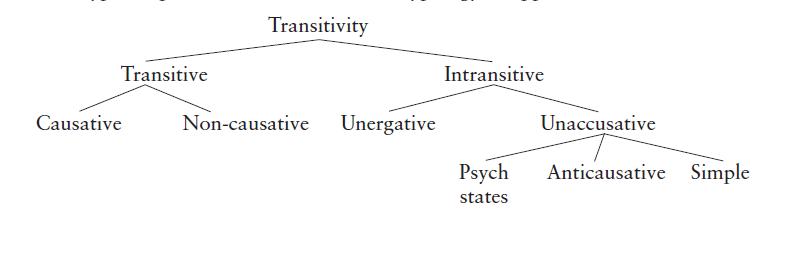
\includegraphics[width=4.5291in,height=1.5563in,width=\textwidth]{cuervo-img001.png}

\end{center}
\begin{styleStandard}
Figure 1: Subtypes of predicates as relevant for a typology of applicatives (Cuervo 2015a: 130)
\end{styleStandard}

\begin{styleStandard}
The classification in Figure 1 predicts some of the contrasts among dative arguments in terms of subtypes of applicatives (such as affected datives with causative verbs versus recipient datives with non-causative transitives). The way the predicates are subdivided, however, does not directly parallel the typology proposed by Pylkkänen (2002, 2008)\footnote{ From this point on, I cite Pylkkänen 2008, but most issues discuss appeared first in Pylkkänen 2002. } and later enriched by Boneh \& Nash 2011, Cuervo 2003, 2010, Kim 2011, McGinnis 2001, 2008, McGinnis \& Gerdts 2004, Roberge \& Troberg 2009, among others. Additionally, the classification based on predicate type does not capture certain proposed implications or correlations among subtypes of applicatives. For instance, if a language allows dative/applicative possessors or recipients with unaccusatives, it also does with transitives, but the reverse does not necessarily hold, as in English. The classification cannot express the intra-linguistic correlation between having (or not having) datives with “lexically” causative verbs (v.g., \textit{break, melt}), and (not) allowing for datives with anticausatives (see Peterson 2007 and Cuervo 2015a for discussion). 
\end{styleStandard}

\begin{styleStandard}
What is needed is a classification based on structural properties directly relevant for the subtypes of applicatives described in the literature, with the potential to systematically derive the interpretation of the various applicatives/datives, and the “natural classes” of crosslinguistic variation in the availability of applicatives.
\end{styleStandard}

\begin{styleStandard}
In Pylkkänen’s work, the crucial distinction in height is actually a distinction between the category or type of the complement of the applicative head\footnote{ This distinction could be reinterpreted in other terms. For example, McGinnis distinguisges symmetrical and asymmetrical applicatives in terms of phases. See also Boneh \& Nash (2017) for a scalar approach to high and low datives in Russian. }. To the basic distinction between applicatives taking nominal complements or entities (LowAppl) and applicatives taking verbal complements or events (HighAppl), further distinctions have been developed, particularly among the verbal complements. 
\end{styleStandard}

\begin{styleStandard}
Kim (2011) proposed that in addition to the applicatives which take verbal complements to the exclusion of the subject (vP), there are those which take a larger verbal projection including the subject (VoiceP). This is the case of Peripheral Applicatives which introduce a nominative affectee in Korean and Japanese passives.\footnote{ In Korean passives, a nominative affectee is the only argument that can trigger honorific agreement with the verb. In the example below, Kim (2012) analyzes \textit{apeci-ka} ‘father’ as a Peripheral Applicative: a high applicative merged above VoiceP.\par 
\setcounter{listWWNumxxvleveli}{0}
\begin{listWWNumxxvleveli}
\item 
\begin{styleFootnote}
\textit{apeci}\textit{\textsubscript{1}}\textit{{}-ka} \ \ \ \ \ \ \textit{Minswu}\textit{\textsubscript{2}}\textit{{}-eykey \ \ pal-ul \ \ \ \ \ \ palp-hi-si}\textit{\textsubscript{1/*2}}\textit{{}-ess-t}
\end{styleFootnote}
\end{listWWNumxxvleveli}
\ \ father-NOM \ Minsu-DAT \ \ \ \ \ \ foot-ACC \ \ step-PASS-HON-PAST-DEC\par \ \ ‘Father\textsubscript{1} was adversely affected by Minsu’s stepping on his\textsubscript{1} foot.’ \ \ (Kim 2012)} Tsai (2018) proposes an even higher applicative for Mandarin, which licenses an argument above the inflectional domain and is “involved in the arrangement of the information strucutre” (Tsai 2018:18). 
\end{styleStandard}

\begin{styleStandard}
Cuervo (2003, 2011, 2015a) proposed that applicative heads taking verbal complements are sensitive to the eventive (dynamic) or stative nature of the vP. Benefactives are prototypical cases of high applicatives taking a dynamic vP as complement; experiencers are prototypical cases of high applicatives taking (psychological) stative vPs. 
\end{styleStandard}

\begin{styleStandard}
Further, in previous work I have argued that the interpretation of applied arguments not only depends on the (type of) complement of the applicative head and properties of the head, but is also affected by the structure \textit{above} the Appl head\footnote{ A reviewer wonders whether this interpretation is countercyclic, and should be restricted to occur within a phase. Indeed, the relevant interpretation discussed here is thematic interpretation at the level of argument structure, which is arguably restricted to the domain limited by VoiceP at the edge. The view that structure above a head is relevant for interpretation, although initially surprising, is compatible with Wood and Marantz’s (2017) unification of argument-introducing heads into one, whose distinct interpretations arise as cases of contextual allosemy, that is, configurational meanings within the extended projection of the verb. See below for discussion.}. Specifically, I have argued that the interpretation of a high applicative is affected by the structure above the applicative phrase, in particular by whether there is another vP above it, embedding or selecting the ApplP, as in the case of Affected Applicatives with (bi-eventive) causatives and anticausatives/inchoatives. For example, Affected Applicatives (3) and Experiencers (4) are both high applicatives which take a stative vP as complement; the predictable contrast in interpretation arises from the Experiencers being non-embedded high applicatives (4c) and the Affected Appl being embedded under a dynamic vP (agentive v\textsc{\textsubscript{do}} in causatives or non-agentive v\textsc{\textsubscript{go}} in inchoatives), as in (3c).
\end{styleStandard}

\begin{styleStandard}
(3) \ \ Affected datives 
\end{styleStandard}

\begin{styleStandard}
a. With causatives: French\ \ 
\end{styleStandard}

\begin{styleStandard}
\ \ \textit{Le teinturier lui a massacré une chemise. }
\end{styleStandard}

\begin{styleStandard}
\ \ the dry-cleaner \textsc{cl.dat} has destroyed a shirt
\end{styleStandard}

\begin{styleStandard}
\ \ ‘The dry-cleaner ruined her/his shirt (on her/him).’ \ (Boneh \& Nash 2012)\ \ \ \ 
\end{styleStandard}

\begin{styleStandard}
b. With anticausatives: Spanish 
\end{styleStandard}

\begin{styleStandard}
\ \ \textit{A Carolina \ \ \ \ se \ \ \ \ \ \ \ \ le \ \ \ \ \ \ \ rompió \ \ la radio }
\end{styleStandard}

\begin{styleStandard}
Carolina.\textsc{dat} \textsc{cl.ref} \textsc{cl.dat} \ \ \ broke \ \ \ \ the radio 
\end{styleStandard}

\begin{styleStandard}
‘The radio broke on Carolina’
\end{styleStandard}

\begin{styleStandard}
c. Structure of Affected Appl in causatives (Cuervo 2003:113)
\end{styleStandard}

\begin{styleStandard}
\ \ \ \ \ \ \ \ \ \ \  \ \ \  \ VoiceP
\end{styleStandard}

\begin{styleStandard}
\ \ \ \  \ \ \ \ 3 \ 
\end{styleStandard}

\begin{styleStandard}
\ \ \ \ \ \ DP\textsubscript{Subj} \ \ \ \ \ 3 \ \textit{v}P
\end{styleStandard}

\begin{styleStandard}
\ \ \ \ \ \ \ \ Voice \ \ \ 3 \ \textbf{ApplP}
\end{styleStandard}

\begin{styleStandard}
\textit{\ \ \ \ \ \ \ \ v}\textsc{\textsubscript{do \ \ \ \ \ }}\ \ \ 3 
\end{styleStandard}

\begin{styleStandard}
\ \ \ \ \ \ \ \  \ \ \ \ \ \ \textbf{DP}\textbf{\textsubscript{Dat}}\textbf{ \ \ \ 3} \ \textbf{\textit{v}}\textbf{P}\textbf{\textsc{\textsubscript{be}}}
\end{styleStandard}

\begin{styleStandard}
\textbf{\ \ \ \ \ \ \ \ \ \ \ \ \ \ \ \ \ \ \ \ \ \ \ \ \ \ \ \ \ \ \ \ \ \ \ \ Appl \ \ \ \ \ \ \ 3 }
\end{styleStandard}

\begin{styleStandard}
\ \ \ \ \ \ \ \ \ \ \ \ \ \ \ \ \ \ \ \ \ \ \ \ \ \ \ \ DP\textsubscript{Obj} \ \ \ \ \textbf{6 }
\end{styleStandard}

\begin{styleStandard}
\textit{\ \  \ \ \ \ \ \ \ \ \ \ \ \ \ \ \  \ \ \ v}+Root\ \ \ \ 
\end{styleStandard}

\begin{styleStandard}
(4) \ \ \ \ Dative experiencers \ \ \ 
\end{styleStandard}

\begin{styleStandard}
a. \ \ \textit{A Rosa \ \ \ \ \ le \ \ \ \ \ \ \ \  \ \ molesta \ \ el humo}
\end{styleStandard}

\begin{styleStandard}
\ \ Rosa.\textsc{dat} \ \ \textsc{cl.dat} \ bother\ \ the smoke
\end{styleStandard}

\begin{styleStandard}
\ \ ‘Smoke bothers Rosa’ \ \ (Acedo-Matellán \& Mateu 2015: 90)
\end{styleStandard}

\begin{styleStandard}
b. \ \ \textit{A Emilio \ \ \ \ \ le parecen \ \ difíciles esas decisiones}
\end{styleStandard}

\begin{styleStandard}
\ \ Emilio.\textsc{dat} \ \textsc{cl.dat} seem \ \ difficult those decisions \ \ 
\end{styleStandard}

\begin{styleStandard}
\ \ ‘Emilio finds those decisions difficult’ 
\end{styleStandard}

\begin{styleStandard}
c. Structure of dative experiencers\ \  
\end{styleStandard}

\begin{styleStandard}
\textbf{ApplP}
\end{styleStandard}

\begin{styleStandard}
\ \ \ \ \ \ \ \ \ \ \ \ 3 
\end{styleStandard}

\begin{styleStandard}
\textbf{\ \ DP}\textbf{\textsubscript{Dat}}\textbf{ }\ \ \ \ \ \ \ \ 3 \ \ \textbf{\textit{v}}\textbf{P}\textbf{\textsc{\textsubscript{be}}}
\end{styleStandard}

\begin{styleStandard}
\ \ \ \ \ \ \ \ \ \ \ \  \ \ \ \ \textbf{Appl} \ \ \ 3 \ 
\end{styleStandard}

\begin{styleStandard}
\ \ \ \ \ \ \ \ \ \ \ \ \ \ \ \ \ \ \ \  \ \ \ \ \ \ DP \ \ \ \ \ \ \ \ \ \ 3 \ 
\end{styleStandard}

\begin{styleStandard}
\textit{\ \ \ \ \  \ \ \ \ \ \ \ \ \ \ \ \ \ \  \ \ \ \ \ \ \ \ \ v}\textsc{\textsubscript{be \ \ \ \ \ \ \ \ }}\ \ \ \ Root\ \  \ (Cuervo 2003: 145)
\end{styleStandard}

\begin{styleStandard}
This way, Affected Applicatives are distinguished from LowAppl by the structure \textit{below} them: they appear above the root, and take a verbal complement. In turn, they are distinguished from Experiencers by the structure \textit{above }them within the extended verbal projection. \ \ \ \ 
\end{styleStandard}

\begin{styleStandard}
The structure above the applicative is also responsible for the contrast between “instrumentals” and “causees”, two types of arguments analyzed as high applicatives taking a dynamic vP as complement. “Causee” is the interpretation assigned to an instrumental high applicative embedded under a dynamic vP (v\textsubscript{cause} \ or v\textsubscript{do}).\footnote{ Some dative causees have been argued to be volitional agents, compatible with agent-oriented adverbials, as in the case of Spanish \textit{hacer}{}-infinitive constructions (parallel to the French \textit{faire}{}-\textit{infinitif}. In this case, there is no agreement whether these should be considered applicatives (as in Torrego 2011) or not (Kim 2011, Tubino 2012). See §4.3 for further discussion.} Unlike an instrumental applicative—embedded directly under Voice which is related to the same event as the agent—a causee is the only external argument related to the embedded event. Although putting together these two types of arguments might initially seem questionable, Jerro observes that “several genetically unrelated and geographically non-contiguous languages have morphological forms that subsume both causative and applicative uses” (Jerro 2017: 752), and proposes for Kinyarwanda a common origin for both types of arguments. \ Kim (2011) proposes an explanation for the causee-instrumental syncretism in Korean and Niuean arguing that “in morphological causatives, a causer uses a causee as an instrument to make a relevant event take place” (2011: 499). According to Kim, the Niuean instrumental applicative morpheme \textit{aki} introduces the causee under causative \textit{faka}{}-. She further observes that in Middle Korean morphological causatives, a causee was marked with the instrumental –(\textit{u)lo}, as illustrated in (5), and that an “animate dative DP in morphological causatives and adversity clauses can also be interpreted as an instrument” (Kim 2011: 499). 
\end{styleStandard}

\begin{styleStandard}
(5) \ \ \textit{ai-lo hwenhi tung-ul kulk-hi-ko}
\end{styleStandard}

\begin{styleStandard}
\ \ child\textsubscript{{}-ACTIVE.INSTR} cool back\textsubscript{{}-ACC} scratch-i-and
\end{styleStandard}

\begin{styleStandard}
\ \ ‘[I] had\textsubscript{caus} my child scratch my back cool [i.e. relieving the \ \ itch].’ \ \ \ \ \ \ \ \ (Park 1994, in Kim 2011:499)
\end{styleStandard}

\begin{styleStandard}
With respect to low applicatives, merged under the verbal root, the distinction between dynamic and stative applicatives also seems to play a role. Pylkkänen defined two sub-types of low applicatives, Low Appl\textsc{\textsubscript{to}}\textsubscript{ }and Appl\textsc{\textsubscript{from}}, based on languages whose double-object constructions require a transfer-of-possession predicate, such as English and, arguably, Hebrew.\footnote{ The verb itself can denote a transfer or it can be a creation verb which is interpreted as a transfer event in combination with a LowAppl. \ } These constructions are doubly dynamic, in the sense that both the transfer predicate (arguably requiring a \textsc{path} structure) and the applicative head encode dynamic relations. \ 
\end{styleStandard}

\begin{styleStandard}
Besides those merged under dynamic verbs of transfer of possession, in some languages a low applicative can also appear under transitive or unaccusative verbs that do not denote \textit{transfer} of possession (either dynamic or stative verbs). This is Cuervo’s (2003) LowAppl\textsc{\textsubscript{at}}, which expresses a non-dynamic possession relation. LowAppl\textsc{\textsubscript{at}} can take \ a DP, a PP or a small clause-type of structure as complement, the applied argument being interpreted as different sub-types of possessors: possessor (6), locative (7), or experiencer (8).
\end{styleStandard}

\begin{styleStandard}
(6) \ \ \ \ a. \ DP complement: possessor dative (transitive; French)
\end{styleStandard}

\begin{styleStandard}
\ \ \textit{Michele \ \ \ lui \ \ \ \ \ \ a lavé \ \ \ \ les cheveux \ \ }
\end{styleStandard}

\begin{styleStandard}
\ \ Michele \ \ \textsc{cl.dat} has washed \ \ the hairs
\end{styleStandard}

\begin{styleStandard}
\ \ ‘Michele washed his hair’ 
\end{styleStandard}

\begin{styleStandard}
\ \ b. \ DP complement: possessor dative (unaccusative; Spanish)
\end{styleStandard}

\begin{styleStandard}
\ \ \textit{A la casa \ \  \ \ le \ \ \ \ faltan \ \ \ \ ventanas }
\end{styleStandard}

\begin{styleStandard}
\ \ the house.\textsc{dat} \textsc{cl.dat} \ \ miss.\textsc{pl}\ \ windows
\end{styleStandard}

\begin{styleStandard}
\ \ ‘The house lacks (some) windows’
\end{styleStandard}

\begin{styleStandard}
(7) \ \ \ \ a. DP-PP complement: locative-possessor dative (Spanish)
\end{styleStandard}

\begin{styleStandard}
\ \ \textit{Gabi \ \ le \ \ \ \ \ \ \ \ puso \ \ el bebé \ \ \ en los brazos \ \ a Emilio}
\end{styleStandard}

\begin{styleStandard}
\ \ Gabi \ \ \ \textsc{cl.dat} put \ \ the baby \ in the arms \ \ \ Emilio.\textsc{dat}\ \ 
\end{styleStandard}

\begin{styleStandard}
\ \ ‘Gabi placed the baby in Emilio’s arms’ 
\end{styleStandard}

\begin{styleStandard}
\ \ b. PP complement: locative-possessor dative (transitive; French)
\end{styleStandard}

\begin{styleStandard}
\ \ \textit{Elle lui \ \ a tiré \ \  \ \ dans le ventre.}
\end{styleStandard}

\begin{styleStandard}
\ \ she \ \textsc{cl.dat} \ \ has shot \ \ in the belly
\end{styleStandard}

\begin{styleStandard}
\ \ ‘She shot her/him in the belly’ \ \ (Boneh \& Nash 2012)
\end{styleStandard}

\begin{styleStandard}
(8) \ \ \ \ a. SC complement: experiencer/locative-possessor dative \ \ (Spanish)
\end{styleStandard}

\begin{styleStandard}
\ \ \textit{Emilio le puso la mano encima a Lucila}\footnote{ Following Cuervo 2003, I assume here that the particle \textit{encima} acts as the predicate in a small-clause-type of structure, which the applicative head takes as its complement. Unlike there, however, I take the datives in (8) to be low applicatives because they are merged as a complement of the verb. See Acedo-Matellán (2017) for an Affected Appl analysis of special datives in Latin.} \textit{\ \ \ \ }
\end{styleStandard}

\begin{styleStandard}
\ \ Emilio.\textsc{nom} \ \textsc{cl.dat} put \ \ the hand on-top \ Lucila.\textsc{dat}\ \ \ \ ‘Emilio laid a hand on Lucila’ 
\end{styleStandard}

\begin{styleStandard}
\ \ b. DP complement: experiencer-possessor dative (Spanish)
\end{styleStandard}

\begin{styleStandard}
\ \ \textit{A Emilio \ \ \ \ \ le \ \ duele una muela \ \ \ \ }
\end{styleStandard}

\begin{styleStandard}
\ \ Emilio.\textsc{dat} \ \textsc{cl.dat} hurt \ \ a molar\ \ 
\end{styleStandard}

\begin{styleStandard}
\ \ ‘Emilio’s molar hurts’ \ 
\end{styleStandard}

\begin{styleStandard}
Sentences (7a-b) show that a dative argument can be the possessor of a body part or location expressed as the DP complement of a preposition. For (7a), a dative co-appearing with a direct object and a locative PP, one can wonder what the complement of the applicative head is, that is, whether the dative takes the [direct object + locative] or just the locative PP as its complement (as it arguably does in (7b)). While it is true that there is a possession relation between the dative and the locative that excludes the direct object (this is evident in the English translation), the entailment of the sentence is expressed as a possessive construction with the dative as external argument and the theme and locative as internal arguments of \textit{tener} ‘have’ (e.g. \textit{Emilio tiene el bebé en (los) brazos} ‘Emilio has the baby on his arms’). \ This shows that the part-whole relation between \textit{Emilio} and \textit{the arms} does not require a syntactic relation between the two to the exclusion of the theme \textit{the baby}.\footnote{ If this were the case, one would expect the entailment to be a location of the theme, expressed as subject, with respect to the dative and PP as internal arguments: \textit{El bebé está en los brazos de Emilio} ‘The baby is on Emilio’s arms’.} \ \ \ \ 
\end{styleStandard}

\begin{styleStandard}
In the examples above, the dative argument is interpreted primarily as the possessor of a body part; in each case, however, there is an “extra” layer of meaning arising from the structure, the meaning of the verb and world knowledge: benefactive (6a), malefactive or affected (7b), locative (6b, 7a), experiencer in (8). 
\end{styleStandard}

\begin{styleStandard}
The interpretation that is secondary in the examples above (affected, experiencer) becomes primary—and the possession interpretation is not entailed, although it might arise as secondary—for other types of dative/applicatives. This is the case of dative experiencers, which are possessors of a mental state, as seen in (4), and Affected Applicatives in (3), which are affected by the change of state of an object (expressed as the direct object). In the case of Affected Applicatives, many times the dative argument is also understood as the possessor of that object, and what aretermed Affected or Middle Applicatives are sometimes classified as possessors (e.g., Fernández Alcalde 2014; see Cuervo 2003 for arguments to distinguish possessors from affected datives both syntactically and semantically). 
\end{styleStandard}

\begin{styleStandard}
As a result of these three distinctions (category of complement, stativity/dynamicity of complement, and embedding structure), a more articulated typology of applicatives can be constructed that accounts for subgroups of applicatives attested in particular languages, as well as the various interpretations that applicative arguments can have inter- and intra-linguistically. Ideally, the typology should also be a good base to account for the morphological form of the Appl head—in particular whether it is overt or null—as well as for the observed syncretisms between applicatives, causatives, adpositions and case markers.
\end{styleStandard}

\begin{styleStandard}
[Warning: Draw object ignored][Warning: Draw object ignored]\ \ \ \ \ \ \ \ Complement
\end{styleStandard}

\begin{styleStandard}
[Warning: Draw object ignored][Warning: Draw object ignored][Warning: Draw object ignored]\ \  \ \ \ \ \ Non-verbal\ \ \ \ \ \  \ \ \ \ \ \ \ \ \ \ \ Verbal (vP)
\end{styleStandard}

\begin{styleStandard}
[Warning: Draw object ignored]
\end{styleStandard}

\begin{styleStandard}
Dynamic (\textsc{to-from}) \ Stative (\textsc{at}) \ \ \ \ \ \ \ \  \ \ \ \ \ \ \ \ 
\end{styleStandard}

\begin{styleStandard}
[\textsc{recipient}] \ \  \ \ \ \ \ \ \ [\textsc{possessor}]
\end{styleStandard}

\begin{styleStandard}
[\textsc{source}]\ \ \ \ \ \ \ \ \ \ \ \ \ \ \ \ \ \  \ \ 
\end{styleStandard}

\begin{styleStandard}
[Warning: Draw object ignored][Warning: Draw object ignored][Warning: Draw object ignored][Warning: Draw object ignored]\ \ \ \ \ \  \ \ \ \ \ \ \ \ \ Dynamic\ \ \ \  \ \ \ \ \ \ \ \ \ \ \ \ \ \ \ \ \ \ \ \ \ \ \ \ \ \ \ \ Stative
\end{styleStandard}

\begin{styleStandard}
[Warning: Draw object ignored][Warning: Draw object ignored][Warning: Draw object ignored][Warning: Draw object ignored]\ \  \ Embedded \ \ \ \ \ \ \ \ Non-embedded\ \  \ \ \ Embedded \ \  \ \ \ \ \ \ \ Non-embedded
\end{styleStandard}

\begin{styleStandard}
\ \  \ \ [\textsc{causee}] \ \ \ \ \ \ [\textsc{instrumental}]\ \ 
\end{styleStandard}

\begin{styleStandard}
\ \ \ \ \ \ \ \ \ \ \ \ \ \ \ \ \ \ \ \ \ \ \ \ \ \ \ \ \ \ \ \ \ \ \ \ \ \ [\textsc{benefactive}]\footnote{ The label \textsc{benefactive} here represents datives with a benefactive, malefactive, or ethical interpretation, as well as ‘substitutive’ applicatives (Peterson 2007).} \ \ Causative \ \ Anticaus\footnote{ I assume here a bi-eventive analysis of anticausative constructions whereby a dynamic event—a vP\textsc{go} expressing the change—embeds a state—a vP\textsc{be} (see Cuervo 2003, 2015b). Thus, an\textsc{ affected} applicative taking a stative vP as complement is embedded under the dynamic vP both in causative and anticausative constructions.} \ Psych \ \ Non-psych \ \ \ \ \ \ \ 
\end{styleStandard}

\begin{styleStandard}
\ \ \ \ \ \  \ \ \ \ \ \  \ \ \ \ \ \ \ \ \ \ [\textsc{affected}] \ \ \ \ \ \ \ \ \ \ \ \ [\textsc{experiencer}]
\end{styleStandard}

\begin{styleStandard}
\textit{Figure 2: Subtypes of applicatives according to their position in structure and properties of their complement}
\end{styleStandard}

\begin{styleStandard}
Figure 2 presents a typology of applicatives organized on the basis of configurational properties. As the diagram represents an inventory of Appl heads, it is possible to associate each node in the tree with particular features on the Appl head, both substantive and selectional. Thus, the splits proposed should reflect intrinsic properties of the Appl head or properties of its complement, but should not reflect properties of the structure that appears above the ApplP (which ‘selects’ the ApplP), as discussed below. Additionally, in an ideal geometry, we would expect that node labels and splits will not repeat within the diagram, and that each division will delineate a particular subtype of Appl. The diagram fulfills this to an important extent, but fails in two places, as discussed below.
\end{styleStandard}

\begin{styleStandard}
The classification in Figure 2 captures Pylkkänen’s idea that there are two types of applicatives. The two types are distinguished mainly in terms of their height within the extended verbal projection, in reference to being above or below the verb (specifically the root). This distinction results in the first split between Appls taking a verbal complement, HighAppl, and a non-verbal complement (but not necessarily a DP), LowAppl.\footnote{ I remain agnostic with respect to the existence of applicatives that merge higher than vP (such as peripheral applicatives proposed by Kim 2011 and Tsai 2018), as opposed to applicatives found outside the extended verbal domain as a result of movement, and, therefore they are not represented n this typology. }
\end{styleStandard}

\begin{styleStandard}
The contrast between dynamicity and stativity is further introduced as a distinction relevant for both applicatives taking verbal and non-verbal complements. Within (non-embedded) high applicatives, this split captures the contrast between \textsc{benefactives} and \textsc{instrumentals}—related to dynamic events—on one hand, and \textsc{experiencers}—related to a state—on the other.\footnote{ As noted by a reviewer, Pylkkänen (2008) argued that benefactive high applicatives can combine with static verbs such as \textit{hold}. This “static verb” is eventive and “dynamic” in the relevant sense, however, as suggested by the reviewer, at least in the context of a benefactive applicative. The notion of “static” is presented in Pylkkänen in opposition to dynamic verbs of transfer.} The label \textsc{experiencer} covers the notion of possessors of (mental) states with psychological or non-psychological predicates (see section 4.4 for data and discussion). Among applicatives embedded under a causative, \textsc{causees} correspond to those taking a dynamic event—analytical causatives in many languages—while \textsc{affected} are those related to a change of state—lexical causatives in many languages, and anticausatives/ inchoatives. 
\end{styleStandard}

\begin{styleStandard}
Given that their complement is non-verbal, the contrast in dynamicity in LowAppl is encoded as a property of the sub-type of LowAppl head itself (\textsc{to} and \textsc{from} are dynamic for \textsc{recipients} and \textsc{sources}, respectively; \textsc{at}, for \textsc{possessors} is a stative relation). The contrast between dynamic and stative low applicatives cannot be obtained by simple reference to the embedding verb. Specifically, a stative Appl-\textsc{at} is compatible with both dynamic, eventive verbs (as for Spanish \textit{wash} and \textit{sell}) and stative verbs (\textit{admire, envy}).\footnote{ In contrast, a stative verb (e.g., \textit{admirar} ‘admire’, \textit{faltar} ‘lack’) is only compatible with a stative applicative (LowAppl\textsc{at}). } In the case of LowAppl, what is either dynamic or stative is the (possessive) relationship between the applicative DP and the theme object DP. 
\end{styleStandard}

\begin{styleStandard}
Another distinction is introduced among verbal (high) applicatives: whether the applicative taking a vP as complement is itself embedded under another (dynamic) vP. As mentioned above, \textsc{causees} and \textsc{affected} applicatives appear between two vPs, in contrast to, for example, non-embedded \textsc{benefactives} and \textsc{instrumentals}, which appear between VoiceP and a dynamic vP. 
\end{styleStandard}

\begin{styleStandard}
The split between non-embedded Appls and Appls embedded under another vP refers to the structure immediately above the ApplP, that is, to the head the Appl is a complement of. It is unusual for a feature of the Appl head to allude to its selecting head or phrase, and this appears to be an imperfection of the typology. \ 
\end{styleStandard}

\begin{styleStandard}
Another instance of reference to the structure selecting for the Appl could be found in Appls that select a non-verbal complement, that is, LowAppl. The issue is that Appl exclusively appears as a complement of a verb: Appl needs a verbal environment either above or below it, as it is incompatible in the nominal domain. \ This means that even if we eliminate explicit reference to selecting structure for Appls taking a verbal complement, there will always be implicit reference to a verbal projection above the LowAppl. This property of the classification, rather than being a problem, expresses a central property of applicatives, as opposed to their close relatives, adpositions. In contrast with adpositions, which can typically appear as PP modifiers in the clausal, verbal and nominal domains, Appl is only licensed in a verbal environment. This could be expressed as a feature or variable that needs valuation by a v feature. This proposal accords with Svenonious’s (2007) treatment of verbs containing an eventive variable \textit{e} that is bound by Tense because Appl islike a more restricted Path PP which also “must be linked to verbal structure, hence ultimately bound by tense” (Svenonious 2007: 35). 
\end{styleStandard}

\begin{styleStandard}
As noted earlier, reference to the structure above Appl seems difficult to reconcile with an attempt to capture the various subtypes of applicatives in terms of a geometry of features encoded by the Appl head. These distinctions are better captured by an approach whereby an Appl head is defined as an introducer of an event participant minimally specified as a possessor(-orientation), with its varying interpretations arising contextually. Section 4 develops this approach by deriving the “typology” in Figure 2 on the basis of configurational properties. Further specification, possibly of a lexical nature, is needed to capture contrasts among low applicatives, and between benefactives and instrumentals. \ 
\end{styleStandard}


\setcounter{listWWNumxxiileveli}{0}
\begin{listWWNumxxiileveli}
\item 
\begin{stylelsSectioni}
Deriving the sub-types
\end{stylelsSectioni}


\setcounter{listWWNumxxiilevelii}{0}
\begin{listWWNumxxiilevelii}
\item 
\begin{stylelsSectionii}
Below the verb: low applicatives
\end{stylelsSectionii}
\end{listWWNumxxiilevelii}
\end{listWWNumxxiileveli}
\begin{styleStandard}
This section briefly discusses the properties of low applicatives which take a non-verbal complement, typically a DP. Arguments of this type of Appl are interpreted as \textsc{recipients}, \textsc{possessors}, \textsc{sources} or \textsc{locations}. 
\end{styleStandard}

\begin{styleStandard}
The contrast among subtypes of LowAppl has been accounted for in terms of subtypes of heads: \textsc{to} and \textsc{from} for recipients and sources, respectively (Pylkkänen 2008) and \textsc{at} for possessors (Cuervo 2003).\footnote{ In some languages, including Spanish, locatives and other special arguments can also be expressed as LowAppl.} Although dynamicity (or directionality) is at the core of the three sub-types, this constrast cannot be simply derived from differences in the complement of the Appl head, or other configurational properties. \ As such, the distinction might require encoding as a feature on the applicative head (+/- dynamic, or [Path], for instance); alternatively, the distinction can be captured as a root element associated with the applicative head (as proposed by Wood \& Marantz 2017 for high applicatives and Prepositions).\footnote{ A reviewer asks whether this difference in encoding is predicted to have empirical consequences. One consequence concerns whether variation in semantics is systematic or unconstrained, which is a central part of my future research. In addition to semantics, intra- and crosslinguistic variation in morphological overtness and shape of heads will be an important topic.} Individual languages could, in principle, choose freely among these heads, although \textsc{to} is the most widespread and basic LowAppl (also the least morphologically marked, Cuervo 2015a).
\end{styleStandard}

\begin{styleStandard}
Although in Pylkkänen (2002, 2008), LowAppl was defined as an applicative merged under a transitive verb expressing transfer of possession, I have shown in previous work that the same relation can take place under unaccusative verbs, as well attested in Spanish with both dynamic verbs (e.g., \textit{crecer} ‘grow’\textit{, caer ‘}fall’\textit{, llegar ‘}arrive’\textit{, doler ‘}hurt’\textsubscript{Intr}) and stative, existential verbs (e.g., \textit{faltar }‘lack’\textit{, quedar ‘}remain’\textit{, sobrar ‘}be\textit{ }extra’), contra Baker (1996). 
\end{styleStandard}

\begin{styleStandard}
The defining feature of low applicatives is therefore their position as complements of the verb and their possession relation (with an entity or location), rather than the transfer meaning, or the transitivity of the verb. With respect to the category of their complement, LowAppls do not necessarily select a DP: all that is required is that they take a non-verbal complement. As such, cases in which an applicative takes a prepositional phrase or a small clause as complement, as illustrated in (7-8), would be cases of low applicatives (LowAppl\textsc{\textsubscript{at}}, specifically).
\end{styleStandard}

\begin{listWWNumxxiileveli}
\item 
\begin{listWWNumxxiilevelii}
\item 
\begin{stylelsSectionii}
Benefactives, instrumentals and other dynamic high applicatives
\end{stylelsSectionii}
\end{listWWNumxxiilevelii}
\end{listWWNumxxiileveli}
\begin{styleStandard}
This section discusses the properties of high applicatives which take a dynamic, eventive vP as complement, and appear under a Voice head. These high applied arguments are typically interpreted as benefactives, malefactives, or instrumentals. 
\end{styleStandard}

\begin{styleStandard}
Benefactives seem to be the most widespread type of high applicatives (Polinsky 2013): applicatives that license an argument related to a dynamic event in a non-actor role. Malefactives and so-called ‘ethical datives’ can be captured in the same way structurally. The different interpretations could be associated with different subtypes of applicative heads, or could be derived as a combination of a ‘factive’ meaning of the Appl head, lexical meaning of the verb, and world knowledge. This seems to be the case for ‘ethical datives’ in Romance (\textit{dativus commodi/incommod}i, see Roberge \& Troberg 2009 for discussion of terms for the various datives labelled ‘ethical’ or ‘dative of interest’), in which arguments with the same morphosyntax can be alternatively understood as benefactives (9a) or malefactives (9b); examples from Roberge \& Troberg 2009.
\end{styleStandard}

\begin{styleStandard}
(9) \ \ \ \ Bene/malefactive applicatives: vP\textsc{do} complement
\end{styleStandard}

\begin{styleStandard}
a. Portuguese benefactive
\end{styleStandard}

\begin{styleStandard}
\textit{\ \ Elle ligou-lhes \ \ \ \ amavelmente a luz}
\end{styleStandard}

\begin{styleStandard}
\ \ he \ \ connected-\textsc{cl.dat.3pl} kindly \ \ the light
\end{styleStandard}

\begin{styleStandard}
\ \ ‘He kindly switched on the light for them’
\end{styleStandard}

\begin{styleStandard}
b. Italian malefactive
\end{styleStandard}

\begin{styleStandard}
\ \ \textit{Gli invitati gli hanno mangiato tutto quello che rimaneva nel frigo. }
\end{styleStandard}

\begin{styleStandard}
\ \ the guests \ \textsc{cl.dat} \ have eaten all that which remained in-the fridge \ 
\end{styleStandard}

\begin{styleStandard}
\ \ ‘The guests ate everything that was left in the fridge on him’
\end{styleStandard}

\begin{styleStandard}
Instrumental applicatives have also been assigned the same structural properties, but are thematically related to the event in a more active initiator or actor-like role. If the same position is assigned to instrumental applicatives, then a featural analysis of argument introducing heads could distinguish them from (bene/male)factives with a +actor/initiator specification. Interestingly, in Kinyarwanda, benefactives and instrumentals are introduced with the same applicative morphology, but contrast in terms of the relative word order between the applicative and the direct object (benefactives appear before, instrumentals after; McGinnis \& Gerdts 2004).
\end{styleStandard}

\begin{styleStandard}
Causees are also introduced by an Appl which takes a dynamic vP as complement. As we have seen, the contrast between instrumentals and causees reduces in this approach to a contrast between being embedded under another dynamic v (Causees) or not (Instrumentals, merged under Voice). Given the semantic and syntactic similarity, and the syncretisms between causatives and instrumentals discussed in section 3 for Niuean, Korean and Kinyarwanda, this is a welcome result.\footnote{Syncretic forms between benefactives and causatives are found in Hualapai (Peterson 2007).} 
\end{styleStandard}

\begin{styleStandard}
This classification, which considers the structure below and above the Appl head, can also capture “accidental causers” in unaccusative change-of-state verbs (inchoatives), as well as non-volitional agents with activity verbs. \ 
\end{styleStandard}

\begin{styleStandard}
In the case of dative arguments with anticausative predicates, a dative argument is usually ambiguous between an affected reading and an unintentional or accidental causer reading. This is the case for Spanish and German, among other languages. Cuervo (2003, 2014) and Schäfer (2008) propose that the accidental causer reading is the interpretation of a high applicative which takes the bi-eventive inchoative structure as its complement (v\textsc{go}{}-v\textsc{be}), and which crucially does not merge under an agentive Voice head (example and structure from Cuervo 2003: 166-7). 
\end{styleStandard}

\begin{styleStandard}
(10) \ \ a. \ \ Dative with inchoative
\end{styleStandard}

\begin{styleStandard}
\textit{Al tintorero se le quemaron los pantalones de Carolina}
\end{styleStandard}

\begin{styleStandard}
\ \ the dry-cleaner\textsc{.dat} \ \textit{\ }\textsc{se} \ \textsc{cl.dat} \ burnt.\textsc{pl} the trousers of Carolina
\end{styleStandard}

\begin{styleStandard}
\ \ ‘Carolina’s trousers got burnt on the dry-cleaners’ or
\end{styleStandard}

\begin{styleStandard}
\ \ ‘The dry-cleaner accidentally burnt Carolina’s trousers’\ \ \ \ 
\end{styleStandard}

\begin{styleStandard}
b.\ \ Structure of accidental causer high applicative
\end{styleStandard}

\begin{styleTextbody}
\ \ \ \ \ \ \ \ \ \ \ \ \ \ \ \ \ \ \ \ \ \ \ \ \textbf{ApplP}
\end{styleTextbody}

\begin{styleStandard}
[Warning: Draw object ignored]\ \ \ \ \textbf{3} 
\end{styleStandard}

\begin{styleStandard}
\ \ \textbf{DP}\textbf{\textsubscript{Dat}}\textbf{ \ \ \ \ \ \ \ 3} \textit{v}P\textsc{\textsubscript{go}}\textsubscript{2}
\end{styleStandard}

\begin{styleStandard}
\ \ \ \ \ \ \ \ \ \ \ \ \ \ \ \ \ \ \ \ \ \ \ \ \ \ \ \ \textbf{Appl} \ \ \ \ \ \ 3 \ \textit{v}P\textsc{\textsubscript{be}}\textsubscript{1}
\end{styleStandard}

\begin{styleStandard}
\ \ \ \ \ \ \ \ \ \ \ \ \ \ \ \ \ \ \ \ \ \ \ \ \ \ \ \ \ \ \ \ \ \ \ \ \ \ \ \ \ \ \ \ \ \ \ \ \textit{v}\textsc{\textsubscript{go }}\textsc{\ \ \ \ \ \ \ \ \ \ \ \ }3 
\end{styleStandard}

\begin{styleStandard}
\ \ \ \ \ \ \ \ \ \ \ \ \ \ \ \ \ \ \ \ \ \ \ \ \  \ \ \ \ \ \ \ \ \ DP\textsubscript{Obj} \ \ \ \ \ \ \ \ 5 \ \ \ 
\end{styleStandard}

\begin{styleStandard}
\textit{\ \ \ \ \ \ \ \ \ \  \ \ \ \ v}+Root
\end{styleStandard}

\begin{styleStandard}
On the same basis, “non-volitional agents” expressed as dative arguments, as in Russian impersonal constructions, could be introduced by a high applicative which takes a dynamic v\textsc{do} as complement, but no Voice head is projected above it.\footnote{ Alternatively, a Voice head is projected but it is somehow defective and does not project an argument in its specifier (morphologically expressed as a reflexive). } Except for the structure above them, these arguments are like instrumentals: an entity or individual involved agentively in an event, but without volition (see Skorniakova 2009 for discussion).
\end{styleStandard}

\begin{styleStandard}
(11)\ \ \textit{Boris-u xorošo pe-l-o-s’ (\# toby zarabota-t’ denegi).}
\end{styleStandard}

\begin{styleStandard}
\ \ Boris\textsc{\textsubscript{dat.masc}} \ \ well sing\textsc{\textsubscript{past-neut-refl}} \ \ in-order make\textsc{\textsubscript{inf}} money
\end{styleStandard}

\begin{styleStandard}
\ \ ‘Boris (felt like) singing well in order to make money.’ \ \ (adapted from Skorniakova 2009:189)
\end{styleStandard}

\begin{listWWNumxxiileveli}
\item 
\begin{listWWNumxxiilevelii}
\item 
\begin{stylelsSectionii}
Embedded high applicatives: affected applicatives and causees
\end{stylelsSectionii}
\end{listWWNumxxiilevelii}
\end{listWWNumxxiileveli}
\begin{styleStandard}
This section briefly discusses the properties of two kinds of high applicatives embedded under a dynamic, eventive vP: those which take another eventive vP as complement (applied DP interpreted as Causee), and those which take a stative vP (their applied argument interpreted as Affected). 
\end{styleStandard}

\begin{styleStandard}
Affected Applicatives are defined as those which appear in change-of-state constructions, both transitive causatives and intransitive anticausative/inchoatives (Cuervo 2003, 2010, 2015b), as illustrated in (3), repeated as (12) below. 
\end{styleStandard}

\begin{styleStandard}
(12) \ \ a. \ \ \ \textit{Le teinturier lui a massacré une chemise. }
\end{styleStandard}

\begin{styleStandard}
\ \ \ \ the dry-cleaner \textsc{cl.dat} has destroyed a shirt
\end{styleStandard}

\begin{styleStandard}
\ \ \ \ ‘The dry-cleaner ruined her/his shirt (on her/him).’ \ (Boneh \& Nash 2012)\ \ \ \ 
\end{styleStandard}

\begin{styleStandard}
b. \ \ \textit{A Carolina \ \ \ \ se \ \ \ \ \ \ \ \ le \ \ \ \ \ rompió \ \ la radio }
\end{styleStandard}

\begin{styleStandard}
\ \ \ \ Carolina.\textsc{dat} \textsc{cl.ref} \textsc{cl.dat} \ \ \ broke \ \ the radio 
\end{styleStandard}

\begin{styleStandard}
\ \ ‘The radio broke on Carolina’
\end{styleStandard}

\begin{styleStandard}
These applicatives take a state as complement and, in this sense, are the “possessors” of a state. In this they resemble experiencer applicatives, which also relate to a state, as expressed by Figure 2. \ As possessors or recipients, they can be confused with low applicatives, but two types of evidence suggest a structural as well as an interpretational difference. First, there are languages (e.g., English) in which double objects/low applicatives are productive, but are systematically disallowed in constructions involving an embedded state, such as causative constructions and resultatives (*\textit{The storm broke them the radio}, *\textit{They drank me the teapot empty}). Secondly, Affected applicatives do not need to be the possessors of the theme, although a possession relation might be an inferred component of the interpretation (see Cuervo 2003 for further arguments). 
\end{styleStandard}

\begin{styleStandard}
As argued in §3, it is the projection above the applicative that distinguishes affected from experiencer applicatives, in particular the fact that there is a dynamic event above Appl that signals the initiation of the state in causatives and inchoatives. An experiencer, by contrast, is the highest argument within the extended verbal projection, as represented in (4c) (see §4.4 for more detailed discussion). \ 
\end{styleStandard}

\begin{styleStandard}
Causees are also derived as a type of high applicative, which, like Affected Appl, is “sandwiched” between two verbal layers.\footnote{ In this sense, Causees are a sub-type of Affected Applicatives. However, I reserve the term Affected Appl for those taking a (verbal) state as complement, as a distinction that may be relevant to capture systematic crosslinguistic variation in the availability of applicative constructions. \ } Unlike Affected Appl, Causees take a dynamic, eventive vP as complement. One of the arguments advanced against analysing causees as applicatives has been the interpretation of causees not only as the entity or individual acted upon (or “affected”) but also as agentive. This is the semantic argument based on which Tubino (2012) rejects an applicative account of Italian and Spanish causees. In fact, Kim’s (2012) conclusion is exactly that the difference in agentivity is what distinguishes high applicatives from arguments of Voice, the contrast being encoded as a feature +/- agentive in the licensing head. Boneh \& Nash (2011) also propose that affectedness is the central meaning of applied arguments, while causees are licenced as regular agents, in the specifier of vP. 
\end{styleStandard}

\begin{styleStandard}
The framework presented here reconciles the affectedness and the agentivity components of the interpretation of causees. On the one hand, affectedness—a prominent interpretation of causees in the “obligation” reading of causatives (as in the Romance \textit{faire infinitif} constructions, Folli \& Harley 2007)—could be derived as the meaning of the High Appl head directly. Alternatively, it can arise as the configurational meaning of an argument that participates in two events: the object of the higher verb \textit{faire} and the ‘instrument’ or ‘bene/malefactive’ of the lower predicate, as in Ippolito’s (2000) applicative analysis and in Affected Appls. On the other hand, the agentive or ‘doer’ interpretation of the relation between the dative causee and the lower event can be derived by the applicative being the highest argument within the extended verbal projection of the lower vP (as in accidental causers with unaccusatives, illustrated in (11) above).\footnote{ The Voice projection that licenses the causer relates it to a \textit{different }vP, which merges above the applicative, and it is typically spelled out by a causative affix or light verb.} In other words, agentivity might arise also as the interpretation of an animate argument DP above a dynamic vP for which Voice is not projected.\footnote{ Tollan and Oxford (2018) argue that external arguments of activity verbs can be licensed either as arguments of Voice (for transitives) or v (for unergatives). In a parallel fashion to dative causees receiving an interpretation associated with Voice, dative experiencers as the highest argument within the extended projection of a stative vP also receive an interpretation as the argument of stative Voice: that of holder of a state (Kratzer 1996). See §4.4 for further discussion of experiencer DPs as applied arguments.} This is possible if the meaning of the applied argument is specified more configurationally than determined by the denotation of the head (see Cuervo 2015a, and Wood \& Marantz 2017). 
\end{styleStandard}

\begin{listWWNumxxiileveli}
\item 
\begin{listWWNumxxiilevelii}
\item 
\begin{stylelsSectionii}
Dative experiencers as stative high applicatives
\end{stylelsSectionii}
\end{listWWNumxxiilevelii}
\end{listWWNumxxiileveli}
\begin{styleStandard}
This section discusses several structural and semantic properties of dative experiencers as the last type of applicative in the typology schematized in Figure 2: unembedded high applicatives which take a stative vP as complement, and introduce the highest argument in the extended verbal projection (that is, Voice is not projected). 
\end{styleStandard}

\begin{styleStandard}
Dative experiencers have received much attention following Belletti and Rizzi’s (1988) seminal work on Romance. An important puzzle they \ recognize is the apparent reversal of the usual thematic mapping: the theme is the nominative subject while the experiencer is coded as object, as illustrated below in Spanish and Pashto. Another important characteristic is the stative nature of dative experiencer constructions.\footnote{ Their stative nature has been claimed to cover even cases of eventive interpretations, such as when the verb is in past tense (see Fábregas \& Marín, this volume), and of psychological expressions with light verbs of movement or transfer of possession (as illustrated in Pashto (14)).}
\end{styleStandard}

\begin{styleStandard}
\ (13) \ \ Spanish\textit{ }
\end{styleStandard}

\begin{styleStandard}
\textit{\ \ A Daniela \ \  le \ \ \  \ \ gustan\ \ las películas} \textit{suecas}\ \ \ \ \ \ Daniela.\textsc{dat} \ \ \textsc{cl.dat} like.PL\ \ the movies Swedish
\end{styleStandard}

\begin{styleStandard}
\ \ ‘Daniela likes Swedish movies’ 
\end{styleStandard}

\begin{styleStandard}
\ \ (Lit. ‘Swedish movies are appealing to Daniela’)
\end{styleStandard}

\begin{styleStandard}
\ (14)\textit{\ \ }Pashto\textit{ }
\end{styleStandard}

\begin{styleStandard}
\textit{\ \ Meena taa \ \ de \ pradi \ \ \ \ khelko na \ \ sharem \ \ \ \ \ \ \ \ wer-z-i} \ \ 
\end{styleStandard}

\begin{styleStandard}
\ \ Meena \textsc{dat} of \ \ strange people \textsc{abl }shyness.\textsc{nom }to.3\textsc{rd}{}-go-3
\end{styleStandard}

\begin{styleStandard}
\ \ ‘Meena feels shy of/from strangers.’ \ \  \ \ \ \ \ \ \ (Babrakzai 1999)
\end{styleStandard}

\begin{styleStandard}
\ \ (Lit. ‘Shyness goes to Meena from strange people.’) \ \ \ \ \ 
\end{styleStandard}

\begin{styleStandard}
The nature and source of dative case has been debated, but here the two central questions are 1) where does the “experiencer” interpretation come from? and 2) what kind of arguments are dative experiencers?
\end{styleStandard}

\begin{styleStandard}
With respect to their interpretation, experiencer datives with psych predicates have been characterized as possessors or locations, or holders of psychological states. Parsons (1995), for instance, subsumes experiencers as a case of the more general “in-ness relation” of subjects of states: “x is \textit{in} s” by observing that “when the verb is one of psychology or perception, the \textit{In}{}-ness relation coincides with (…) the Experiencer relation” (1995: 664). For Landau (2010), experiencers are locations of mental states. In de Miguel’s (2015) words, experiencers “combine the values of location and possession” (2015: 243; my translation). This characterization of the meaning of dative experiencers in terms of possessors or locations of states resembles characterizations of stative low applicatives, and makes dative experiencers good candidates for an applicative analysis. Cuervo (2003, 2011) developed a high applicative analysis of dative experiencers: the experiencer DP is external to the state specified by the verbal root, of which the nominative DP is the holder. In this sense, there are two “subjects” in the construction in (15).\footnote{ Other evidence that the nominative argument is also a ‘subject’ is that psychological verbs taking dative experiencers are acceptable without the experiencer, in which case the nominative DP typically appears pre-verbally, as illustrated in (i). See Cuervo 2011 for further arguments and data.\par 
\setcounter{listWWNumxxvileveli}{0}
\begin{listWWNumxxvileveli}
\item 
\begin{styleFootnote}
\textit{Los ruidos de la calle no importan/ molestan/gustan}. \ 
\end{styleFootnote}
\end{listWWNumxxvileveli}
\ \ \ \ \ \ \ \ \ the noises of the street not matter/ bother/ appeal\par \ \ \ \ \ \ \ \ \ \ \ \ \ \ \ ‘Street noise is not important/ bothersome/ appealing.’} Dative case and morphological expression of the Appl head as a pronominal clitic are the usual forms for applicative constructions in Spanish. 
\end{styleStandard}

\begin{styleStandard}
(15) Dative experiencers as high applicatives (for example (13)
\end{styleStandard}

\begin{styleNormalWeb}
\ \  \ \ \ \ \ \ \ \ \  \ \ ApplP
\end{styleNormalWeb}

\begin{styleStandard}
\ \ \ \ \ \ \ \ \ \textsc{\textsubscript{\ }}\ \ \ 3 
\end{styleStandard}

\begin{styleStandard}
\ \ \ \ \textbf{DP}\textbf{\textsubscript{Dat}} \ \ \ \ \ \ \ \ \ 3 \ \ \textbf{\textit{v}}\textbf{P}\textbf{\textsc{\textsubscript{be}}}
\end{styleStandard}

\begin{styleStandard}
\ \ \ \ \textit{a Daniela} \ \ \ \ \ \ Appl \ \ \ \ \ \ \textbf{3 }\ 
\end{styleStandard}

\begin{styleStandard}
\ \ \ \ \ \ \ \ \ \ \ \ \ \ \ \ \ \ \ \ \ \ \textit{le} \ \ \ \ \ \ \ \ DP \ \ \ \ \ \ \ \ \textbf{3 \ }\ 
\end{styleStandard}

\begin{styleStandard}
\textit{\ \ \  \ \ \ \ \ \ \ \ \ \  \ \ \ \ \ \ las películas \ \ \ v}\textsc{\textsubscript{be \ \ \ \ \ \ \ \ \ \ \ \ \ \ }}Root 
\end{styleStandard}

\begin{styleStandard}
\ \ \ \ \ \  \ \ \ \ \ \ \ \ \ \ \ \  \ \ \textit{gust}{}-\ \ \ \ 
\end{styleStandard}

\begin{styleStandard}
The high applicative analysis contrasts with previous analyses that equate (the initial position of) dative experiencers with datives in canonical ditransitive constructions, whether treated as double-object, incorporation, low applicative constructions or locatives (Belletti and Rizzi 1988, Masullo 1992, among others).\textsuperscript{ }\footnote{ Acedo-Matellán \& Mateu 2015, Pujalte 2015 adopt the unaccusative analysis with the dative experiencer as HighAppl and the usual dative case (but change the licensing position of the lower DP). }\ \ Unlike those analyses, (15) expresses the fact that the dative DP is not directly related to the other argument, and that there is no possession relation between the two DPs: crucially, the “possession” relation is between the dative DP and the state (the vP complement of the Appl head). 
\end{styleStandard}

\begin{styleStandard}
Dative experiencer constructions reveal semantic crosslinguistic variation based on availability of particular constructions. The structure and meaning of the transitive English sentence \textit{Daniela likes Swedish movies} contrast with its translation equivalent in a language with dative experiencers as in (13), in which the psych predicate expresses a property of the nominative argument (\textit{Las películas suecas gustan}, ‘Swedish movies are appealing’), a predication that is lacking in the English sentence.\footnote{ Not all psych constructions display this variation, however. English also has psych constructions formed with prepositional phrases, such as \textit{to}{}-DPs with psych predicates such as \textit{appeal}, \textit{seem}, and \textit{be important}.} 
\end{styleStandard}

\begin{styleStandard}
As mentioned earlier, experiencers are related to possessors and (human) locations, but are not taken to be affected arguments. This is consistent with the proposal that affectedness in dative or applicative arguments arises as a configurational meaning involving two verbal layers. However, proposing that dative experiencers are unembedded high applicatives which take a stative vP as complement does not directly derive the ‘experiencer’ interpretation. In principle, the interpretation could arise as a result of the lexical meaning of the psych verb, of the denotation of the Appl head or some other specialized head, or the extended verbal configuration as a whole. 
\end{styleStandard}

\begin{styleStandard}
It could be argued that the meaning of the experiencer as a specialized type of possessor or location arises from the meaning of the psych verb, in virtue of the dative DP being one of its arguments. Regardless of whether one has any general reservations against a lexically-based approach to argument structure, there are empirical arguments against deriving the interpretation of the dative experiencer from the lexical meaning of a verb. These arguments are presented below fromSpanish, but other languages provide similar evidence. 
\end{styleStandard}

\begin{styleStandard}
First, not every experiencer is the subject of a \textit{psychological }experience, there also being physical states associated to an experiencer argument, as in (16).\footnote{ The interpretation of the dative in (16) and (19) is not perfectly captured by its English translation. As in the case of other applicatives, such as low and affected applicatives, a dative argument is understood as more than a goal or location, and typically only animate entities are licensed (therefore, the dative in (16) could not be replaced by \textit{the mannequin}) or inanimate entities in a part-whole relation, as in (19b). The contrast between Spanish (16) and its English translation is perhaps similar to the contrast in English between \textit{That is important to Amir/*the lawn} and \textit{That is important for Amir/the lawn}.} Second, intra- and inter-linguistically, many experiencers appear with psychological predicates formed as light verb constructions in which the psych meaning comes from a nominal element, not from the verb, and the dative argument is arguably associated with the light verb, as in (17), and in (14) above. Finally, as noted by di Tullio (2015), there are dative DPs interpreted as experiencers in combination with idiomatic psychological expressions formed without any psych words, as in (18). 
\end{styleStandard}

\begin{styleStandard}
(16) \ \ \textit{A Daniela \ \ le \ \  \ aprietan\ \ los zapatos} 
\end{styleStandard}

\begin{styleStandard}
\ \ Daniela.\textsc{dat} \textsc{cl.dat} squeeze.\textsc{pl }\ \ the shoes
\end{styleStandard}

\begin{styleStandard}
\ \ ‘Those shoes are too tight for Daniela’
\end{styleStandard}

\begin{styleStandard}
(17) \ \ \textit{A Daniela \ \ le \ \  \ dan \ \ \ \ miedo\ \ las tormentas} 
\end{styleStandard}

\begin{styleStandard}
\ \ Daniela.\textsc{dat} \textsc{cl.dat} give.\textsc{pl}\ \ fear\ \ the storms 
\end{styleStandard}

\begin{styleStandard}
\ \ ‘Daniela is afraid of storms’ lit., ‘Storms give fear to Daniela’
\end{styleStandard}

\begin{styleStandard}
(18) \ \ \textit{A Daniela le \ \ dan cosa/ \ \ no sé qué las arañas }
\end{styleStandard}

\begin{styleStandard}
\ \ Daniela.\textsc{dat} \ \ \textsc{cl.dat} give.\textsc{pl }thing/ not know.1\textsc{sg} what the spiders 
\end{styleStandard}

\begin{styleStandard}
\ \ ‘Daniela feels uneasy about spiders’ 
\end{styleStandard}

\begin{styleStandard}
\ \ Lit., ‘Spiders give Daniela stuff/I don’t know what’ (adapted from Di \ \ Tullio 2015)
\end{styleStandard}

\begin{styleStandard}
These data provide evidence against a lexical source of the experiencer interpretation, since experiencers do not require a lexical psychological verb. An alternative explanation is that the interpretation derives directly from the denotation of a specialized, more functional head, whose contribution is to licence an experiencer both syntactically and semantically (as Voice does for Agents). Within an applicative approach, this head would be the Appl head. It can be proposed that there is a specialized Experiencer ‘flavour’ or feature specification of HighAppl (as has been proposed for LowAppl in order to derive the recipient, source and possessor interpretation). A specialized head, rather than the verb, as the source of the experiencer interpretation has also been proposed by Landau (2010), and argued by Fábregas \& Marín (this volume): a prepositional head P which takes the dative DP as its argument and relates it to the state. The non-psychological experiencers illustrated in (16) are potential problems for this “all-in-the-head” approach, since it is not clear whether these cases would require a different P head than the one which combines with psychological predicates. Additional issues arise with arguably experiencer arguments that are hard to classify as either psychological or physical, particularly in the case of inanimate datives, as in (19b). \ \ 
\end{styleStandard}

\begin{styleStandard}
(19) \ \ a. \ \ \textit{A Daniela \ \ le \ \ quedan mal\ \ los zapatos} 
\end{styleStandard}

\begin{styleStandard}
\ \ \ \ Daniela.\textsc{dat} \textsc{cl.dat} stay.\textsc{pl }bad\ \ the shoes
\end{styleStandard}

\begin{styleStandard}
\ \ \ \ ‘Those shoes look bad on Daniela’
\end{styleStandard}

\begin{styleStandard}
\ \ b. \ \ \textit{Al regalo\ \  \ \ \ \ le \ \ queda mal\ \ ese moño}
\end{styleStandard}

\begin{styleStandard}
\ \ \ \ the present.\textsc{dat} \textsc{cl.dat} stay bad\ \ that bow 
\end{styleStandard}

\begin{styleStandard}
\ \ \ \ ‘That bow looks bad on the present’\ \ \ \ \ \ \ \ \ \ 
\end{styleStandard}

\begin{styleStandard}
Even more importantly, a problem with the proposal that experiencer is the meaning assigned by a dedicated applicative (or P) head is that, as noted by Wechsler (this volume), an unconstrained quantity of different heads would be required to account for the other interpretations. The resulting system would be unable to express or account for the systematicity between the structure of the verbal domain and interpretation of arguments. \ \ 
\end{styleStandard}

\begin{styleStandard}
A third, intermediate possibility can be developed within a more explanatory applicative analysis: “experiencer” is a configurational meaning which takes into account the Appl head and its position within the extended verbal projection, properties of the complement of Appl, as well as idiosyncratic meanings of vocabulary items, and idiomatic expressions.\footnote{ Such a configurational approach could also be developed on the basis of Landau’s (2010) functional P head, but I do not pursue that line here. See Acedo-Matellán \& Mateu (2015) for an account of properties of psychological predicates based on characteristics of the root. } Ideally, the semantic contribution of the Appl head is minimal and constant as far as the interpretation of its argument is concerned, although Pylkkänen’s (2008) distinction between High and Low in terms of semantic composition must be maintained.
\end{styleStandard}

\begin{styleStandard}
As specifiers of a high applicative, dative experiencers are related to a vP, and share properties with bene/malefactives, instrumentals, causees, and affected applicatives (Figure 2). Unlike bene/malefactives, Affected Appls and causees, experiencers are not typically affected arguments. Unlike instrumentals, experiencers are not related to an event in a ‘doer’ capacity; if anything, they are closer to undergoers than to agents. Can these different interpretations be derived without postulating “experiencer” directly as the denotation of a particular HighAppl head?
\end{styleStandard}

\begin{styleStandard}
As discussed in section 3, experiencers are structurally distinguishable from both Affected Appls and Causees, as represented in Figure 2 by the “embedded/non-embedded” contrast. Since affectedness arises from the applicative argument participating in two (sub)events, the lack of affectedness reading for dative experiencers follows. The contrast between experiencers and bene/malefactives and instrumentals is based, in Figure 2, on the dynamic or stative nature of the complement vP. Stativity is a crucial component of our understanding (or definition) of an experiencer as the possessor of a mental state. Another property of the structure of dative experiencer constructions, however, is crucial: the experiencer is the highest argument, there not being another external argument licensing head (such as v or Voice) above Appl. 
\end{styleStandard}

\begin{styleStandard}
In order to test whether these two structural components are needed to obtain an “experiencer” reading (of a high applicative), they should be isolated. First, stative verbs that are not unaccusative, such as Spanish \textit{vivir} ‘live’, usually appear in unergative structures with a nominative subject alone, or with a locative as well. A dative argument may be added to the sentence with a locative, as in (20).\footnote{ The resulting sentence is colloquial, and not accepted by all speakers. In any case, the relevance of the example is the interpretation obtained by those speakers who accept it. }
\end{styleStandard}

\begin{styleStandard}
(20)\ \ \textit{Emilio le vive en el jardín} (\textit{a Vera}). 
\end{styleStandard}

\begin{styleStandard}
\ \ Emilio \textsc{cl.dat} \ \ live in the garden (Vera.\textsc{dat)}
\end{styleStandard}

\begin{styleStandard}
\ \ ‘Emilio is living in Vera’s garden (on her)’
\end{styleStandard}

\begin{styleStandard}
The interpretation of the dative argument \textit{Vera} in (20) is not that of an experiencer, but more specifically a bene/malefactive, arguably due to the presence of the external argument, merged above the high applicative, which, in turn, takes a stative vP as complement. 
\end{styleStandard}

\begin{styleStandard}
The other test is an unaccusative structure in which the dative is the highest argument, but in which the vP complement is dynamic rather than stative. Would such dative be interpreted as an experiencer? \ Fábregas \& Marín (this volume) probe this question and suggest that a dative argument with a reflexive dynamic predicate i a potential experiencer:
\end{styleStandard}

\begin{styleStandard}
(21) \ \ \textit{A Juan se le olvidan las cosas (rápidamente)}.
\end{styleStandard}

\begin{styleStandard}
\ \ Juan.\textsc{dat} \textsc{se cl.dat} forget.\textsc{pl} the things quickly
\end{styleStandard}

\begin{styleStandard}
\ \ ‘Juan forgets things (quickly)
\end{styleStandard}

\begin{styleStandard}
This sentence is in present tense, just like the typical stative in (13), but here the present is understood as episodic or habitual, as an activity verb would. Interestingly, what Fábregas \& Marín consider an experiencer could be the result of the psychological nature of the predicate in an inchoative structure, in which a dative argument would typically be read as an accidental causer. This highlights the interaction between structural properties and lexical meaning in the interpretation of a dative DP. Note in the examples below how the interpretation of the dative is somewhat different in the absence of a psychological reading of the predicate. In the unintentional causer reading, the underlying structure is that of a high applicative merged above a (non agentive) dynamic vP\textsc{go} (Cuervo 2003, 2014; Schäfer 2008; see §4.2).
\end{styleStandard}

\begin{styleStandard}
(22) \ \ \textit{A Juan se le pierden/queman las cosas}. 
\end{styleStandard}

\begin{styleStandard}
\ \ Juan.\textsc{dat} \textsc{se cl.dat} \ \ lose.\textsc{pl} / burn.\textsc{pl}\ \ the things
\end{styleStandard}

\begin{styleStandard}
\ \ ‘Juan (accidentally) loses/burns things’ 
\end{styleStandard}

\begin{styleStandard}
These data support the view that the interpretation of a (dative) argument as an “experiencer” is better captured as a configurational meaning rather than a meaning dependent on the denotation of a licensing head or a lexical element. In particular, the data show that both stativity of the verbal complement, and absence of an external argument above the dative DP, are crucial components for the experiencer interpretation to arise as the most salient.\footnote{ Kim’s (2011) analysis of Korean adversity passives as experiencer \textit{have} constructions (as in English \textit{Peter had the children laugh at him}) is also crucially based on the “affected experiencer” being the highest external argument in the extended verbal domain. Interestingly, these two properties also hold of the arguably other way of licensing experiencer subjects: as Holder arguments licensed by Voice in the context of a psychological predicate, as in \textit{Natasha fears lighting}. \ }
\end{styleStandard}


\setcounter{listWWNumxxiileveli}{0}
\begin{listWWNumxxiileveli}
\item 
\begin{stylelsSectioni}
Conclusions
\end{stylelsSectioni}
\end{listWWNumxxiileveli}
\begin{styleStandard}
Classical Nahuatl grammarian Horacio Carochi characterized applicatives as those which “orient the action of the verb towards another person, or thing, attributing it to him by way of harm, or benefit, taking it away from him, or putting it on him, or relating it to him in some way or another, as shall be understood through the examples; e.g., \textit{nitlaqua}, ‘I eat something’; its applicative is \textit{nictlaquaia in notàtsin}, ‘I eat my father something’, as if he has fruit, or something else, and I eat it from him...”: 
\end{styleStandard}

\begin{styleStandard}
VERBO aplicativo es el que ordena la acción del verbo a otra persona, o cosa, atribuyéndosela por via de daño, o provecho, quitándosela, o poniéndosela, o refiriéndosela de qualquiera manera que sea, como se entenderá por los exemplos; verbi gracia: \textit{nitlaqua}, ‘como algo’, su aplicativo es \textit{nictlaquaia in notàtsin}, ‘como algo a mi Padre’, como si tenía fruta, o otra cosa, y se la como. (Carochi 1645: 466)
\end{styleStandard}

\begin{styleStandard}
Carochi’s translation of the Náhuatl applicative into Spanish involved the addition of a dative argument (\textit{a mi Padre}, and \textit{se} in \textit{se la como} above), \ illustrating the overlap between applicative and dative arguments. Although the overlap may be imperfect, it is significant and systematic. The study of datives as applicatives provides a framework to capture datives as a class beyond their morphology in terms of the type of licensing, while allowing for systematic variation in terms of structural position and thematic interpretation. 
\end{styleStandard}

\begin{styleStandard}
This broader approach to the study of dative constructions goes well beyond the most typical datives in ditransitive constructions. By putting aside case as a domain where languages can vary, I have focused on what dative arguments have in common as a class and as subcases of applicative arguments, as found in both languages with a rich case system and languages without overt case marking. Going beyond morphosyntactic coding is necessary in the quest to make crosslinguistic generalizations and to articulate a theory of argument structure.
\end{styleStandard}

\begin{styleStandard}
Carochi’s (1645) notion of applicatives as derived verbs captures the intuition that there must be some extra piece in a verb that co-occurs with—and licenses—an applied argument. In order to systematically derive the subtypes of dative/applied arguments, it is crucial to take into account the way this extra piece integrates into the extended verbal projection of the clause. In describing its integration, not only the merge position (i.e., the complement) of the Appl head is relevant, but also the dynamic/stative nature of its complement, and the presence/absence of an external argument, and of a verbal head (intruducing a (sub)event) above the applicative. Once such a detailed proposal is developed, broad empirical coverage can be maintained while featural and lexical specification of the Appl head is drastically reduced. This minimal notion of Appl as introducing an argument “oriented” towards its complement accords well with the fact that in so many languages applicatives are expressed as dative arguments, analyzed themselves as an argument “in contact” with the rest of the predicate (Fábregas \& Marín, this volume) via a directional or locative morpheme, such as Romance \textit{a/à}. Appl is thus akin to the more grammatical adpositions whose complement is interpreted contextually (Svenonious 2007). In this view of semantically underspecified Appl, a distinction remains between applied arguments and arguments of Voice (cf. Wood \& Marantz 2017). 
\end{styleStandard}

\begin{styleStandard}
The richness of interpretations of applicative and dative arguments, in spite of their being licensed by a functional head with minimal semantics, sets them apart from the narrow range of interpretations for arguments of \textit{v}/Voice, on the one hand, and the practically unconstrained interpretations of arguments of lexical verbs/roots, on the other. Applicatives are, in this sense, an “efficient” way of generating diversity of meaning with limited resources by making use of various properties of the syntactic structures with which they combine.
\end{styleStandard}

\begin{styleStandard}
\textbf{References}
\end{styleStandard}

\begin{styleStandard}
Acedo-Matellán, Víctor. 2017. Latin datives with prefixed verbs and beyond: A view from the theory of applicatives. \textit{Catalan Journal of Linguistics} 16: 19–49.
\end{styleStandard}

\begin{styleStandard}
Acedo-Matellán, Víctor \& Jaume Mateu. 2015. Los verbos psicológicos: raíces especiales en estructuras corrientes. In Rafael Marín (ed.) \textit{Los predicados psicológicos, }81–109. Madrid: Visor.
\end{styleStandard}

\begin{styleStandard}
Babrakzai, Farooq. 1999. Topics in the syntax of Pashto. Doctoral dissertation, University of Hawai.
\end{styleStandard}

\begin{styleStandard}
Baker, Mark. 1996. On the structural position of themes and goals. In Johan Rooryck and Laurie Zaring (eds.), \textit{Phrase Structure and the Lexicon}, 7–34. Dordrecht: Kluwer.
\end{styleStandard}

\begin{styleStandard}
Belletti, Adriana, and Luigi Rizzi. 1988. Psych-verbs and[202F?]$\theta ${}-Theory. \textit{Natural Language and Linguistic Theory} 6 (3): 291–352. https://doi.org/10.1007/BF00133902.
\end{styleStandard}

\begin{styleStandard}
Boneh, Nora \& Nash, Lea. 2011. High and higher applicatives: The case of French non-core datives. In \textit{Proceedings of the 28th West Coast Conference on Formal Linguistics}, 60–68. \url{http://www.lingref.com/cpp/wccfl/28/paper2436.pdf}.
\end{styleStandard}

\begin{styleStandard}
Boneh, Nora and Lea Nash. 2013. Core and non-core datives. In Beatriz Fernández \& Ricardo Etxepare (eds.) \textit{Variation in datives: a microcomparative perspective}, 22–49. Oxford: Oxford University Press. 
\end{styleStandard}

\begin{styleStandard}
Boneh, Nora \& Nash, Lea. 2017. The syntax and semantics of dative DPs in Russian ditransitives. \textit{Natural language and linguist theory }35: 899–953. 
\end{styleStandard}

\begin{styleStandard}
Bruening, Benjamin. 2010. Ditransitive asymmetries and a theory of idiom formation. \textit{Linguistic Inquiry} 41:519–562.
\end{styleStandard}

\begin{styleStandard}
Carochi, Horacio. 1645. El arte de la lengua mexicana con la declaración de los adverbios della. Mexico: Museo Nacional de México. (Reprint)
\end{styleStandard}

\begin{styleStandard}
Carrier, Julien. 2014. Applicatives in Inuktitut and transitivity. Ms., University of Toronto.
\end{styleStandard}

\begin{styleStandard}
Cuervo, María Cristina. 2003. \ Datives at large. Doctoral dissertation, MIT.
\end{styleStandard}

\begin{styleStandard}
Cuervo, María Cristina. 2010. \ Against ditransitivity. \textit{Probus} 22, 151–180.
\end{styleStandard}

\begin{styleStandard}
Cuervo, María Cristina. 2011. \ Some dative subjects are born, some are made. In Claudia Borgonovo, Manuel Español-Echevarría and Philippe Prévost (eds.), \textit{Selected Proceedings of the Hispanic Linguistic Symposium 2008}, 26–37. Somerville, Mass.: Cascadilla Press. 
\end{styleStandard}

\begin{styleStandard}
Cuervo, María Cristina. 2014. Alternating unaccusatives and the distribution of roots. \textit{Lingua} 141, 48–70. https://doi.org/10.1016/j.lingua.2013.12.001.
\end{styleStandard}

\begin{styleStandard}
Cuervo, María Cristina. 2015a. Parameters in argument structure II: causatives and applicatives. In Antonio Fábregas, Jaume Mateu and Michael T. Putnam (eds.),\textit{ Contemporary Linguistic Parameters}, 123-145. London: Bloomsbury Academic.
\end{styleStandard}

\begin{styleStandard}
Cuervo, María Cristina. 2015b. Causation without a cause. \textit{Syntax} 18 (4), 388–424. https://doi.org/10.1111/synt.12115.
\end{styleStandard}

\begin{styleStandard}
De Miguel, Elena. 2015. Los nombres psicológicos: propuesta de análisis en términos sub-léxicos. In Rafael Marín (ed.) \textit{Los predicados psicológicos, }211–248. Madrid: Visor.
\end{styleStandard}

\begin{styleStandard}
Demonte, Violeta. 1995. Dative alternation in Spanish. \textit{Probus} 7, 5–30.
\end{styleStandard}

\begin{styleStandard}
Diaconescu, Rodica. 2004. Romanian applicative constructions. Doctoral dissertation, University of Ottawa.
\end{styleStandard}

\begin{styleStandard}
Di Tullio, Ángela. 2015. Variantes sintéticas y analíticas de los predicados psicológicos. In Rafael Marín (ed.) \textit{Los predicados psicológicos,} 185{}-210. Madrid: Visor.
\end{styleStandard}

\begin{styleStandard}
Etxepare, Ricardo \& Bernard Oyharçabal. 2013. Datives and adpositions in Northeastern Basque. In Beatriz Fernandez and Ricardo Etxepare (eds.), \textit{Variation in datives: a microcomparative perspective}, 50-95. Oxford: Oxford University Press. DOI:10.1093/acprof:oso/9780199937363.003.0003
\end{styleStandard}

\begin{styleStandard}
Fernández Alcalde, Héctor. (2014). Two types of datives in Spanish: Caused possession vs. possessor raising. \textit{Acta Linguistica Hungarica} Vol. 61(1): 69–90. DOI: 10.1556/ALing.61.2014.1.3
\end{styleStandard}

\begin{styleStandard}
Folli, Raffaella \& Heidi Harley. 2006. \ Benefactives aren’t goals in Italian. In Jenny Doetjes and Paz González (eds.), \textit{Romance Languages and Linguistic Theory 2004: Selected Papers from Going Romance,} 121-142. Amsterdam: John Benjamins Publishing.
\end{styleStandard}

\begin{styleStandard}
Folli, Raffaella \& Heidi Harley. 2007. Causation, obligation, and argument structure: On the nature of little v. \textit{Linguistic Inquiry} 38 (2), 197–238. \url{https://doi.org/10.1162/ling.2007.38.2.197}.
\end{styleStandard}

\begin{styleStandard}
Fournier, David. 2010. La structure du prédicat verbal: Une étude de la construction à double objet en français. Doctoral Dissertation, University of Toronto.
\end{styleStandard}

\begin{styleStandard}
Grimm, Scott. 2011. \ Semantics of case. \textit{Morphology} 21, 515-544.
\end{styleStandard}

\begin{styleStandard}
Kim, Kyumin. 2011. High Applicatives in Korean causatives and passives. \textit{Lingua} 121 (3), 487–510. \url{https://doi.org/10.1016/j.lingua.2010.10.001}.
\end{styleStandard}

\begin{styleStandard}
Kim, Kyumin. 2012. Affectees in subject position and applicative theory. \textit{The Canadian Journal of Linguistics / La Revue Canadienne de Linguistique} 57 (1): 77–107. \textstyleInternetlink{https://doi.org/10.1353/cjl.2012.0002}.
\end{styleStandard}

\begin{styleStandard}
Kratzer, Angelika. 1996. Severing the external argument from its verb. In Johan Rooryck and Laurie Zaring (eds.), \textit{Phrase structure and the lexicon}, 109–137. Dordrecht: Kluwer.
\end{styleStandard}

\begin{styleStandard}
Harley, Heidi. 2013. External arguments and the mirror principle: On the distinctness of Voice and v. \textit{Lingua} 125: 34–57.
\end{styleStandard}

\begin{styleStandard}
Ippolito, Michela. 2000. Remarks on the argument structure of Romance causatives. Ms., MIT.
\end{styleStandard}

\begin{styleStandard}
Jerro, Kyle. 2017. The causative-instrumental syncretism. \textit{Journal of Linguistics 53}, 751–788. DOI:10.1017/S0022226717000044. 
\end{styleStandard}

\begin{styleStandard}
Landau, Idan. 2010. \textit{The locative syntax of experiencers. }Cambridge, Mass: MIT Press.
\end{styleStandard}

\begin{styleStandard}
Maling, Joan. 2001. Dative: The heterogeneity of the mapping among morphological case, grammatical functions, and thematic roles. \textit{Lingua} 111: 419–464.
\end{styleStandard}

\begin{styleStandard}
Marantz, Alec. 2013. Verbal argument structure: Events and participants. \textit{Lingua} 130: 152–168. http://dx.doi.org/10.1016/j.lingua.2012.10.012
\end{styleStandard}

\begin{styleStandard}
Masullo, Pascual. 1992. Incorporation and case theory in Spanish: A crosslinguistic perspective. Doctoral dissertation, University of Washington. 
\end{styleStandard}

\begin{styleStandard}
McGinnis, Martha. 2001. Variation in the phase structure of applicatives. \textit{Linguistic Variation Yearbook} 1 (1): 105–46.
\end{styleStandard}

\begin{styleStandard}
McGinnis, Martha. 2004. Lethal ambiguity. \textit{Linguistic inquiry} 35.1, 47-95.
\end{styleStandard}

\begin{styleStandard}
McGinnis, Martha. 2008. Applicatives. \textit{Language and Linguistics Compass} 2 (6), 1225–45. \url{https://doi.org/10.1111/j.1749-818X.2008.00078.x}.
\end{styleStandard}

\begin{styleStandard}
McGinnis, Martha. 2018. Applicatives. Ms., University of Victoria.
\end{styleStandard}

\begin{styleStandard}
McGinnis, Martha, and Donna B. Gerdts. 2004. A phase-theoretic analysis of Kinyarwanda multiple applicatives. \url{http://prism.ucalgary.ca/handle/1880/44523}.
\end{styleStandard}

\begin{styleStandard}
Miyagawa, Shigeru, and Takae Tsujioka. 2004. Argument structure and ditransitive verbs in Japanese. \textit{Journal of East Asian Linguistics} 13 (1): 1–38.
\end{styleStandard}

\begin{styleStandard}
Moreno Villamar, Itziri. 2018. Variation in the pronominal clitic system of P'urhépecha-Spanish bilinguals. Doctoral dissertation, Western University.
\end{styleStandard}

\begin{styleStandard}
Park, Jeong-Woon. 1994. Morpholgoical causatives in Korean: Problems in grammatical polysemy and constructional relations. Doctoral dissertation, University of California, Berkeley.
\end{styleStandard}

\begin{styleStandard}
Parsons, Terence. 1995. Thematic relations and arguments. \textit{Linguistic Inquiry} 26 (4): 635–62.
\end{styleStandard}

\begin{styleStandard}
Peterson, David A. 2007. \textit{Applicative constructions}. Oxford: Oxford University Press.
\end{styleStandard}

\begin{styleStandard}
Pineda, Anna. 2016. \textit{Les fronteres de la (in)transitivitat: Estudi dels aplicatius en llengües romàniques i basc} [published and revised version of the doctoral dissertation]. Barcelona: Institut d'Estudis Món Juïc.
\end{styleStandard}

\begin{styleStandard}
Polinsky, Maria. 2013. Applicative constructions. In Matthew Dryer \& Martin Haspelmath (eds.), The world atlas of language structures online. \ Leipzig: Max Planck Institute for Evolutionary Anthropology.
\end{styleStandard}

\begin{styleStandard}
Pujalte, Mercedes. 2009. Condiciones sobre la introducción de argumentos: el caso de la alternancia dativa en español. Master’s thesis, Universidad Nacional del Comahue.
\end{styleStandard}

\begin{styleStandard}
Pujalte, Mercedes. 2015. Hacia un análisis unificado de los predicados psicológicos estativos en español. In Rafael Marín (ed.), \textit{Los predicados psicológicos, }111-144. \ Madrid: Visor.
\end{styleStandard}

\begin{styleStandard}
Pylkkänen, Liina. 2000. What applicative heads apply to. \textit{University of Pennsylvania Working Papers in Linguistics} 7.1(18): 197–210. 
\end{styleStandard}

\begin{styleStandard}
Pylkkänen, Liina. 2002. Introducing arguments. Doctoral dissertation, \ MIT.
\end{styleStandard}

\begin{styleStandard}
Pylkkänen, Liina. 2008. \textit{Introducing arguments}. Cambridge, Mass.: MIT Press.
\end{styleStandard}

\begin{styleStandard}
Roberge, Yves \& Michelle Troberg. 2009. \ The high applicative syntax of the dativus commodi/incommodi in Romance\textit{.}\textbf{\textit{ }}\textit{Probus} 21, 249–289. DOI 10.1515/prbs.2009.008
\end{styleStandard}

\begin{styleStandard}
Schäfer, Florian. 2008. \textit{The Syntax of (Anti-)Causatives: External Arguments in Change-of-State Contexts}. Linguistik Aktuell = Linguistics Today, v. 126. Amsterdam: John Benjamins.
\end{styleStandard}

\begin{styleStandard}
Skorniakova, Oxana. 2009. Syntactic and Semantic properties of Russian dative {\textquotedbl}subjects{\textquotedbl}. In Anastasia Smirnova, Vedrana Mihaliček, and Lauren Ressue (eds.), \textit{Formal Studies in Slavic Linguistics}, 166-196. Cambridge: Cambridge Scholars Publishing.
\end{styleStandard}

\begin{styleStandard}
Svenonious, Peter. 2007. \ Adpositions, particles, and the arguments they introduce. In Eric Reuland, Tanmoy Bhattacharya, and Giorgos Spathas (eds.), \textit{Argument Structure}, 63-103. Amsterdam: John Benjamins. 
\end{styleStandard}

\begin{styleStandard}
Tollan, Rebecca and Will Oxford. 2018. Voice-less unergatives: Evidence from Algonquian. In Wm. G. Bennett, Lindsay Hracs, and Dennis Ryan Storoshenko (eds.), \textit{Proceedings of the 35th West Coast Conference on Formal Linguistics}, 399-408. Somerville, Mass.: Cascadilla Proceedings Project.
\end{styleStandard}

\begin{styleStandard}
Torrego, Esther. 2011. Variability in the case patterns of causative formation in Romance and its implications. \textit{Linguistic Inquiry} 41(3): 445-470.
\end{styleStandard}

\begin{styleStandard}
Tsai, Wei-Tien D. 2018. High applicatives are not high enough: a cartographic solution. \textit{Lingua Sinica} 4:2, 1-21. https://doi.org/10.1186/s40655-018-0034-y
\end{styleStandard}

\begin{styleStandard}
Tubino, Mercedes. 2012. \ Spanish dative causees: against an applicative analysis. Paper presented at the \textit{22nd Colloquium on Generative Grammar}, Universitat Autonoma de Barcelona.
\end{styleStandard}

\begin{styleStandard}
Wood, Jim, and Alec Marantz. 2017. The Interpretation of external arguments. In Roberta D’Alessandro, Irene Franco \& Ángel J. Gallego (eds.), \textit{The verbal domain}, 255–278. Oxford: Oxford University Press. DOI: \url{https://doi.org/10.1093/oso/9780198767886.003.0011}\href{https://www.glossa-journal.org/articles/10.5334/gjgl.527/print/main-text-B65}{\textstyleInternetlink{~}}
\end{styleStandard}

\end{document}
